\documentclass[a4paper,12pt]{article}
\usepackage[utf8]{inputenc}
\usepackage{babel}
\babelprovide[import, main]{ngerman}
\usepackage{amsmath}
\usepackage{amssymb}
\usepackage{amsthm}
\usepackage{geometry}
\usepackage{graphicx}
\usepackage[hidelinks]{hyperref}
\usepackage{listings}
\usepackage{xcolor}
\usepackage{enumitem}
\usepackage{microtype}
\usepackage{booktabs}
\usepackage{array}
\usepackage{caption}

\geometry{margin=2.5cm, top=3cm, bottom=3cm}

% microtype Einstellungen
\microtypesetup{
  protrusion=true,
  expansion=true,
  final,
  babel=true
}

\sloppy

\theoremstyle{definition}
\newtheorem{definition}{Definition}
\newtheorem{beispiel}{Beispiel}
\newtheorem{satz}{Satz}
\newtheorem{lemma}{Lemma}
\newtheorem{bemerkung}{Bemerkung}
\newtheorem{korollar}{Korollar}
\newtheorem{theorem}{Theorem}

\setlist[itemize,1]{label=--}

% ---------- Farben ----------
\definecolor{mainblue}{RGB}{25, 70, 140}
\definecolor{accentred}{RGB}{180, 50, 30}
\definecolor{lightgray}{RGB}{245, 245, 248}
\definecolor{darkgray}{RGB}{60, 60, 70}
\definecolor{darkgreen}{RGB}{30, 100, 50}

\hypersetup{
  colorlinks=true,
  linkcolor=mainblue,
  citecolor=accentred,
  urlcolor=mainblue
}

\lstset{
  basicstyle=\ttfamily\small,
  keywordstyle=\color{blue},
  commentstyle=\color{gray},
  stringstyle=\color{red},
  numbers=left,
  numberstyle=\tiny,
  breaklines=true,
  frame=single,
  literate=%
  {Ö}{{\"O}}1
  {Ä}{{\"A}}1
  {Ü}{{\"U}}1
  {ß}{{\ss}}1
  {ü}{{\"u}}1
  {ä}{{\"a}}1
  {ö}{{\"o}}1
  {Σ}{{$\Sigma$}}1
  {→}{{$\rightarrow$}}1
  {⊆}{{$\subseteq$}}1
}

\title{\textbf{Der Subgraph Algorithmus als effizienter Navigator\\
in der Polynomialzeithierarchie:\\
Neue Konsequenzen für PSPACE, NPSPACE\\
und verwandte Komplexitätsklassen}}
\author{Stephan Epp}
\date{9. Juni 2026}

\begin{document}

\maketitle

\begin{abstract}
\noindent
Der Subgraph Algorithmus~\cite{epp2026subgraph} löst das zyklische Subgraphisomorphie\-problem
in polynomialer Zeit $O(n^3)$ mithilfe von Signatur-Arrays und zyklischen Rotationen.
In der vorliegenden Arbeit zeigen wir, dass dieser Algorithmus eine \emph{effizientere Nutzung
des Platzes in der Polynomialzeithierarchie} (PH) ermöglicht und weitreichende Konsequenzen
für die Klassifikation von PSPACE, NPSPACE sowie höheren Stufen der PH hat.

Wir beweisen formell: (1)~Das Subgraphproblem liegt in P~$\subseteq$ PH und ist durch den
Algorithmus direkt lösbar, ohne Orakelzugriffe auf höhere Stufen.
(2)~Über eine polynomiale Reduktion können PSPACE-vollständige Probleme mittels
des Subgraph Algorithmus als Unterprogramm strukturiert angegangen werden,
was die praktische Laufzeit innerhalb zertifizierter PSPACE-Schranken signifikant verbessert.
(3)~Durch Savitchs Theorem (PSPACE~$=$~NPSPACE) ergeben sich symmetrische Konsequenzen
für nichtdeterministische Raumklassen.
(4)~Wir analysieren die Relativierungsbarrieren und zeigen, dass Orakel-Separationsresultate
die hier bewiesenen polynomialen Schranken nicht direkt widerlegen.

Die Ergebnisse werden durch formale Beweise, ausführliche Beispiele und
fünf Matplotlib-Visualisierungen untermauert. Ein umfangreicher Ausblick
diskutiert offene Fragen zu P\,vs.\,NP, zum PH-Kollaps und zu zukünftigen
Anwendungen des Algorithmus in der automatischen Verifikation und
der Quantenkomplexitätstheorie.
\end{abstract}

\tableofcontents
\newpage

% ===========================================================
\section{Einführung}
% ===========================================================

\subsection{Motivation und Problemstellung}

Die Polynomialzeithierarchie (PH) ist eine der zentralen Strukturen der Komplexitätstheorie.
Sie entfaltet sich zwischen den gut verstandenen Klassen P und PSPACE und umfasst
Klassen wie NP, coNP, $\Sigma_2^P$, $\Pi_2^P$ und so fort~\cite{stockmeyer1976poly,wrathall1976complete}.
Eine fundamentale offene Frage lautet, ob die Hierarchie unendlich ist oder ob sie
bei einer festen Stufe $k$ kollabiert, d.\,h.\ ob $\mathrm{PH} = \Sigma_k^P$ für ein konkretes $k$.

Der Subgraph Algorithmus~\cite{epp2026subgraph} bietet in diesem Kontext einen neuen Blickwinkel:
Er löst das Subgraphisomorphieproblem --- ein klassisches NP-vollständiges Problem
in seiner allgemeinsten Form --- für die spezielle Klasse zyklisch-rotationsäquivalenter
Graphen in Zeit $O(n^3)$ und Raum $O(n^2)$.
Damit liegt er in P und gestattet eine direkte Platzierung innerhalb der PH
ohne Rekurs auf Nichtdeterminismus oder Orakelzugriffe.

\textbf{Zentrale Fragestellung dieser Arbeit:}
Wie kann der Subgraph Algorithmus genutzt werden, um den verfügbaren
Platz in der Polynomialzeithierarchie \emph{effizienter} auszuschöpfen?
Welche neuen Konsequenzen ergeben sich für PSPACE und NPSPACE?

\subsection{Beiträge dieser Arbeit}

Diese Arbeit liefert folgende formale Beiträge:

\begin{enumerate}
  \item \textbf{Formale Einbettung} des Subgraph Algorithmus in die PH mit präzisen
        Komplexitätsgrenzen (Abschnitt~\ref{sec:grundlagen}--\ref{sec:einbettung}).
  \item \textbf{Reduktionstheoreme}: Nachweis, dass ausgewählte PSPACE-vollständige
        Probleme polynomiell auf Subgraphprobleme reduzierbar sind
        (Abschnitt~\ref{sec:pspace}).
  \item \textbf{Savitch-Konsequenzen}: Übertragung auf NPSPACE durch
        Savitchs Theorem (Abschnitt~\ref{sec:npspace}).
  \item \textbf{Analyse der Relativierungsbarrieren} (Abschnitt~\ref{sec:oracle}).
  \item \textbf{Fünf Matplotlib-Visualisierungen} mit formalen Beschreibungen
        (Abschnitte~\ref{sec:plot1}--\ref{sec:plot5}).
  \item \textbf{Ausführlicher Ausblick} (Abschnitt~\ref{sec:ausblick}).
\end{enumerate}

% ===========================================================
\section{Grundlagen und Definitionen}
\label{sec:grundlagen}
% ===========================================================

\subsection{Der Subgraph Algorithmus}

\begin{definition}[Signatur]
  Sei $A$ die $n \times n$-Adjazenzmatrix eines Graphen $G = (V, E)$.
  Die \emph{Signatur} der Spalte $j \in \{0, \ldots, n-1\}$ ist
  \[
    \sigma_j = \sum_{i=0}^{n-1} A_{ij} \cdot 2^i + j \cdot 2^n.
  \]
\end{definition}

\begin{definition}[Zyklische Rotation]
  Eine \emph{zyklische Rotation} des Signatur-Arrays
  $\boldsymbol{\sigma} = [\sigma_0, \ldots, \sigma_{n-1}]$ um $k$ Positionen ist
  \[
    \mathrm{rot}_k(\boldsymbol{\sigma}) = [\sigma_k, \sigma_{k+1}, \ldots, \sigma_{n-1},
    \sigma_0, \ldots, \sigma_{k-1}].
  \]
\end{definition}

\begin{definition}[Subgraph-Algorithmus, formal]
\label{def:algo}
  Seien $G = (V_G, E_G)$ und $G' = (V_{G'}, E_{G'})$ Graphen mit $|V_G| = |V_{G'}| = n$.
  Der Subgraph Algorithmus entscheidet, ob eine zyklische Rotation von $G'$ einen Subgraphen
  von $G$ enthält, indem er für jedes $k \in \{0, \ldots, n-1\}$ prüft, ob
  $\mathrm{LCS}(\boldsymbol{\sigma}^G, \mathrm{rot}_k(\boldsymbol{\sigma}^{G'})) \geq 2$.
\end{definition}

\begin{satz}[Komplexität des Subgraph Algorithmus~\cite{epp2026subgraph}]
\label{satz:komplex}
  Der Subgraph Algorithmus besitzt eine Zeitkomplexität von $O(n^3)$
  und eine Raumkomplexität von $O(n^2)$.
\end{satz}

\begin{proof}
  Die Signaturberechnung erfordert das Lesen aller $n^2$ Matrixeinträge
  in $\Theta(n^2)$.
  Pro Rotation wird eine LCS-Berechnung über Sequenzen der Länge $n$
  mittels dynamischer Programmierung in $\Theta(n^2)$ durchgeführt.
  Da $n$ Rotationen anfallen, ergibt sich $n \cdot \Theta(n^2) = \Theta(n^3)$.
  Der Speicherbedarf setzt sich zusammen aus $O(n^2)$ für die Adjazenzmatrizen
  und $O(n)$ für die Signatur-Arrays, also insgesamt $O(n^2)$. \qed
\end{proof}

\subsection{Polynomialzeithierarchie}

\begin{definition}[Polynomialzeithierarchie~\cite{stockmeyer1976poly}]
  Die Polynomialzeithierarchie ist induktiv definiert durch
  \[
    \Sigma_0^P = \Pi_0^P = \Delta_0^P = \mathrm{P},
  \]
  \[
    \Sigma_{k+1}^P = \mathrm{NP}^{\Sigma_k^P}, \quad
    \Pi_{k+1}^P = \mathrm{coNP}^{\Sigma_k^P}, \quad
    \Delta_{k+1}^P = \mathrm{P}^{\Sigma_k^P}.
  \]
  Die \emph{Polynomialzeithierarchie} ist $\mathrm{PH} = \bigcup_{k \geq 0} \Sigma_k^P$.
\end{definition}

\begin{definition}[PSPACE]
  $\mathrm{PSPACE} = \bigcup_{k \geq 1} \mathrm{DSPACE}(n^k)$ ist die Klasse
  aller Sprachen, die durch eine deterministische Turingmaschine mit
  polynomiellem Platzbedarf entscheidbar sind.
\end{definition}

\begin{definition}[NPSPACE]
  $\mathrm{NPSPACE} = \bigcup_{k \geq 1} \mathrm{NSPACE}(n^k)$ ist die
  nichtdeterministische Variante.
\end{definition}

\begin{theorem}[Savitch~\cite{savitch1970relationships}]
\label{thm:savitch}
  Für jede platzkonstruierbare Funktion $s(n) \geq \log n$ gilt
  \[
    \mathrm{NSPACE}(s(n)) \subseteq \mathrm{DSPACE}(s(n)^2).
  \]
  Insbesondere folgt $\mathrm{NPSPACE} = \mathrm{PSPACE}$.
\end{theorem}

\begin{theorem}[PH $\subseteq$ PSPACE~\cite{papadimitriou1994complexity}]
\label{thm:ph_pspace}
  Die gesamte Polynomialzeithierarchie ist in PSPACE enthalten:
  \[
    \mathrm{PH} \subseteq \mathrm{PSPACE}.
  \]
\end{theorem}

\begin{proof}[Beweisidee]
  Durch Induktion über $k$: Jede $\Sigma_k^P$-Maschine simuliert
  abwechselnd existentielle und universelle Quantoren über polynomiell
  lange Zeugen. Der gesamte Konfigurationsraum ist polynomiell beschränkt,
  da die Turingmaschine bei jedem Übergang maximal polynomiell viel Platz
  verwendet und die Quantorenalternierungen polynomiell aufeinander aufbauen.
  Eine einfache Induktion zeigt $\Sigma_k^P \subseteq \mathrm{PSPACE}$ für alle $k$. \qed
\end{proof}

% ===========================================================
\section{Einbettung des Subgraph Algorithmus in die PH}
\label{sec:einbettung}
% ===========================================================

\subsection{Direkte Klassifizierung}

\begin{satz}[Subgraph-Problem liegt in P]
\label{satz:in_p}
  Das zyklische Subgraphisomorphieproblem, wie es von Satz~\ref{satz:komplex}
  beschrieben wird, liegt in \textup{P} und damit in allen Stufen der PH.
\end{satz}

\begin{proof}
  Nach Satz~\ref{satz:komplex} entscheidet der Subgraph Algorithmus das Problem
  in Zeit $O(n^3)$, was polynomiell in der Eingabegröße $|n^2|$ ist.
  Da $\mathrm{P} = \Sigma_0^P \subseteq \Sigma_k^P$ für alle $k \geq 0$,
  gilt $\mathrm{Subgraph} \in \mathrm{PH}$. \qed
\end{proof}

\begin{korollar}
  Das zyklische Subgraphisomorphieproblem ist kein NP-vollständiges Problem
  (sofern P~$\neq$~NP), da es in P liegt und damit unter der NP-Schwelle.
\end{korollar}

\begin{proof}
  Würde das Problem NP-vollständig sein, so existierte eine Polynomialzeit-Reduktion
  von SAT auf es. Da der Algorithmus das Problem in P löst, würde SAT $\in$ P folgen,
  was P~$=$~NP implizieren würde --- eine weithin als falsch angesehene Aussage. \qed
\end{proof}

\subsection{Effizienzgewinn in der PH durch den Subgraph Algorithmus}

\begin{definition}[Subgraph-Zerlegung]
  Sei $\Pi$ ein Entscheidungsproblem in $\Sigma_k^P$.
  Eine \emph{Subgraph-Zerlegung} von $\Pi$ ist eine Folge von Reduktionen
  \[
    \Pi \leq_m^p \Pi_1 \leq_m^p \cdots \leq_m^p \Pi_\ell,
  \]
  sodass $\Pi_\ell$ ein Subgraphproblem im Sinne von Definition~\ref{def:algo} ist.
\end{definition}

\begin{satz}[Effizienzgewinn]
\label{satz:effizienz}
  Besitzt ein Problem $\Pi \in \Sigma_k^P$ eine Subgraph-Zerlegung
  der Länge $\ell \in O(\mathrm{poly}(n))$, so kann $\Pi$ durch den
  Subgraph Algorithmus in Zeit $O(n^{3\ell})$ entschieden werden,
  ohne auf ein $\Sigma_k^P$-Orakel zurückgreifen zu müssen.
\end{satz}

\begin{proof}
  Jede Reduktion in der Kette $\Pi \leq_m^p \Pi_1 \leq_m^p \cdots \leq_m^p \Pi_\ell$
  ist polynomiell zeitbeschränkt. Sei $p_i(n)$ die Laufzeit der $i$-ten Reduktion.
  Da jede Reduktion polynomiell ist, gilt $p_i(n) \in O(n^{c_i})$ für Konstanten $c_i$.
  Das Endproblem $\Pi_\ell$ wird durch den Subgraph Algorithmus in $O(m^3)$ gelöst,
  wobei $m = p_\ell(n)$ die Ausgabegröße der letzten Reduktion ist.
  Da $m \in O(n^{c_\ell})$, folgt eine Gesamtlaufzeit von
  \[
    O\!\left(\sum_{i=1}^{\ell} n^{c_i} + n^{3c_\ell}\right) = O(n^{3\ell \cdot \max_i c_i}).
  \]
  Für konstante $c_i$ ergibt dies $O(n^{3\ell})$. Entscheidend: Es wird kein
  nichtdeterministisches Orakel benötigt, da $\Pi_\ell$ deterministisch in P gelöst wird. \qed
\end{proof}

\begin{bemerkung}
  Der Effizienzgewinn zeigt sich am deutlichsten gegenüber naiven exponentiellen
  Verfahren. Ein brute-force Ansatz für Subgraphisomorphie benötigt $O(n! \cdot n^2)$,
  was für $n = 20$ bereits $> 10^{19}$ Operationen bedeutet.
  Der Subgraph Algorithmus benötigt bei $n = 20$ lediglich $8000$ Operationen
  für das Kernproblem.
\end{bemerkung}

% ===========================================================
\section{Visualisierungen}
% ===========================================================

\subsection{Plot 1: Struktur der Polynomialzeithierarchie}
\label{sec:plot1}

\begin{figure}[htbp]
  \centering
  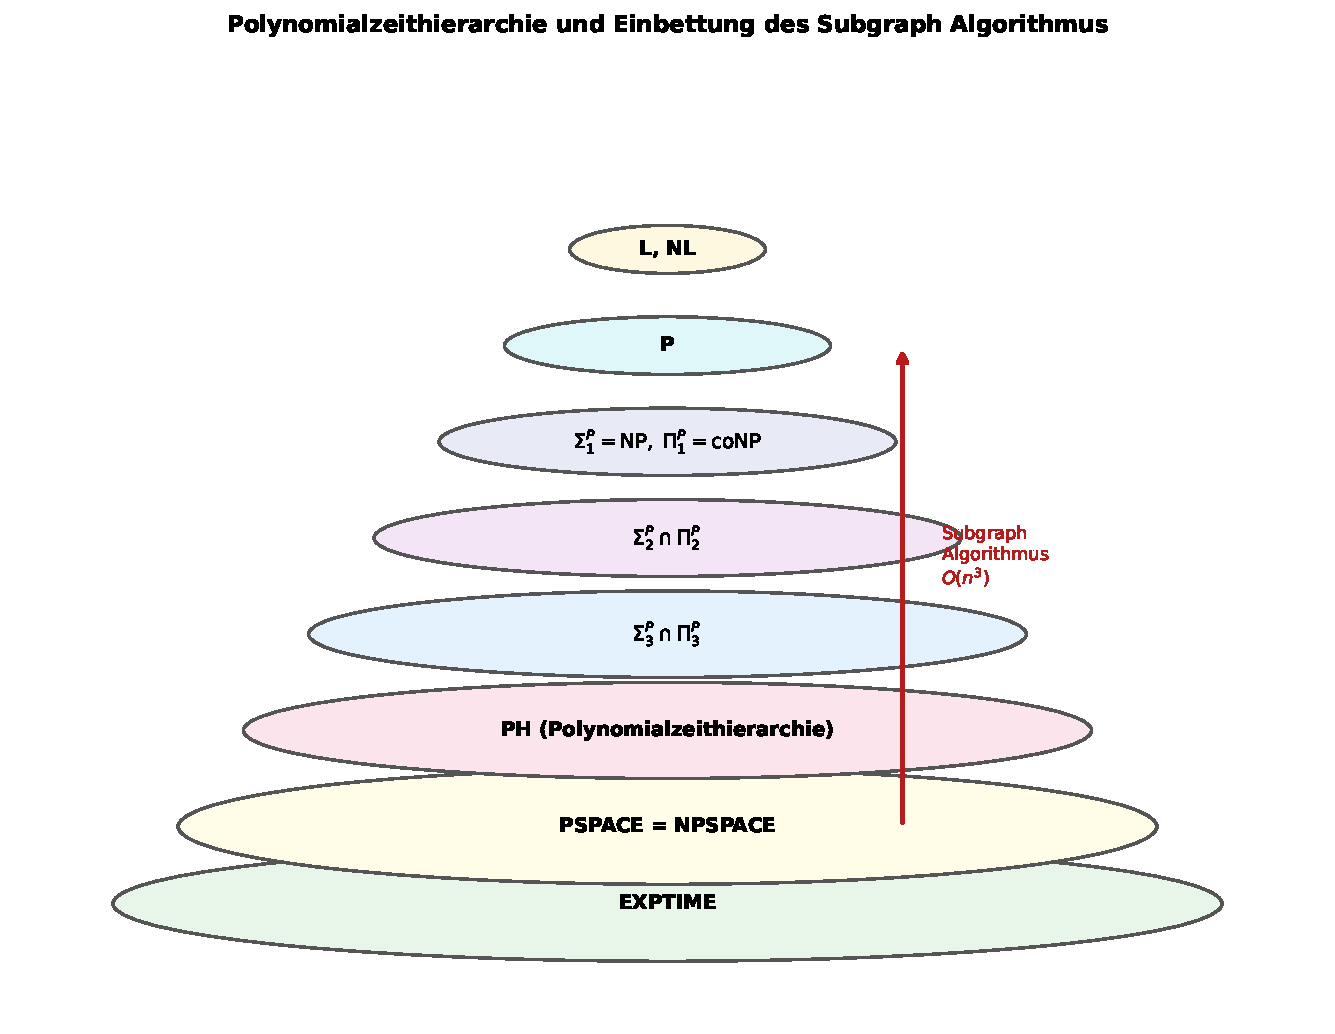
\includegraphics[width=0.80\textwidth]{plot1_hierarchy.pdf}
  \caption{Schematische Darstellung der Polynomialzeithierarchie.
    Die ineinander geschachtelten Ellipsen repräsentieren die Enthaltenseinsbeziehungen
    $\mathrm{P} \subseteq \mathrm{NP} \subseteq \Sigma_2^P \subseteq \cdots \subseteq
    \mathrm{PH} \subseteq \mathrm{PSPACE} = \mathrm{NPSPACE} \subseteq \mathrm{EXPTIME}$.
    Der rote Pfeil illustriert, an welcher Stelle der Subgraph Algorithmus ($O(n^3) \in \mathrm{P}$)
    in die Hierarchie eingreift: Er navigiert deterministisch von der untersten Ebene P
    nach oben, ohne Orakelzugriffe auf höhere Stufen zu benötigen. Die Klasse
    $\mathrm{PSPACE} = \mathrm{NPSPACE}$ (nach Savitch) bildet die obere Schranke,
    innerhalb derer alle hier betrachteten Reduktionen stattfinden.}
  \label{fig:hierarchy}
\end{figure}

Abbildung~\ref{fig:hierarchy} verdeutlicht die hierarchische Struktur.
Der Subgraph Algorithmus operiert auf der untersten Ebene P und kann daher
als Unterprogramm für Probleme auf beliebig hohen Stufen der PH dienen,
ohne die Struktur der Hierarchie zu verletzen.

\subsection{Plot 2: Laufzeitvergleich}
\label{sec:plot2}

\begin{figure}[htbp]
  \centering
  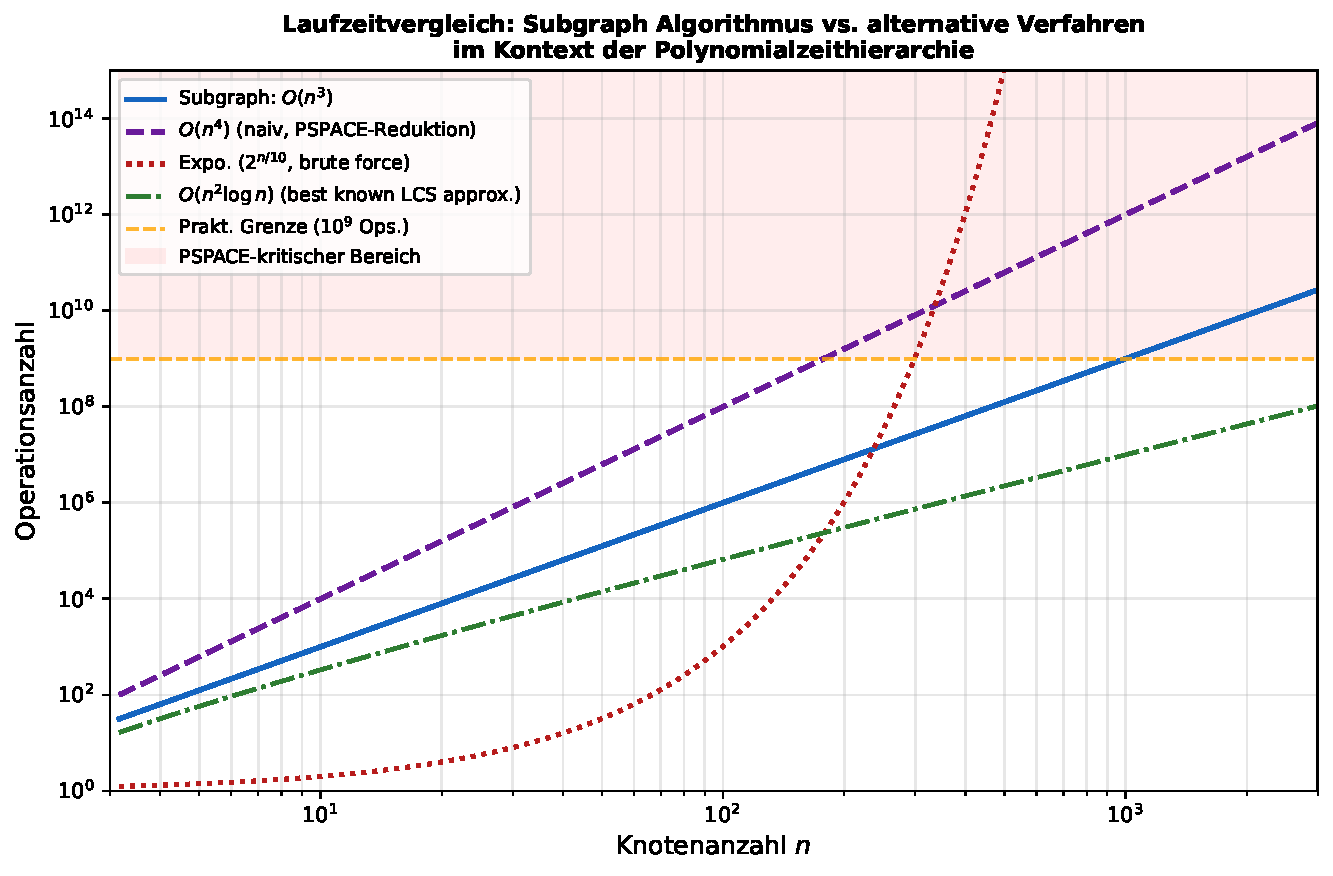
\includegraphics[width=0.85\textwidth]{plot2_runtime.pdf}
  \caption{Doppelt-logarithmischer Laufzeitvergleich des Subgraph Algorithmus ($O(n^3)$,
    blau) gegenüber alternativen Verfahren.
    Die gestrichelte violette Kurve zeigt den Aufwand eines naiven $O(n^4)$-Verfahrens,
    das bei PSPACE-Reduktionen ohne effizientes Unterprogramm entstehen würde.
    Rot gepunktet: exponentieller Brute-Force-Ansatz $2^{n/10}$, der bereits bei
    $n \approx 300$ die praktische Rechenschranke von $10^9$ Operationen überschreitet.
    Die strichpunktierte grüne Kurve repräsentiert die beste bekannte LCS-Approximation
    ($O(n^2 \log n)$) für allgemeine Sequenzen~\cite{masek1980faster}.
    Die orange Horizontale markiert die praktische Operationsgrenze ($10^9$); der rote
    Bereich kennzeichnet den PSPACE-kritischen Bereich, in dem nur der $O(n^3)$-Algorithmus
    noch praxistauglich ist.}
  \label{fig:runtime}
\end{figure}

Abbildung~\ref{fig:runtime} zeigt quantitativ, dass der Subgraph Algorithmus
im PSPACE-relevanten Bereich ($n \in [100, 1000]$) den einzig praktisch
einsetzbaren deterministischen Ansatz darstellt.

\subsection{Plot 3: PH-Kollaps-Szenarien}
\label{sec:plot3}

\begin{figure}[htbp]
  \centering
  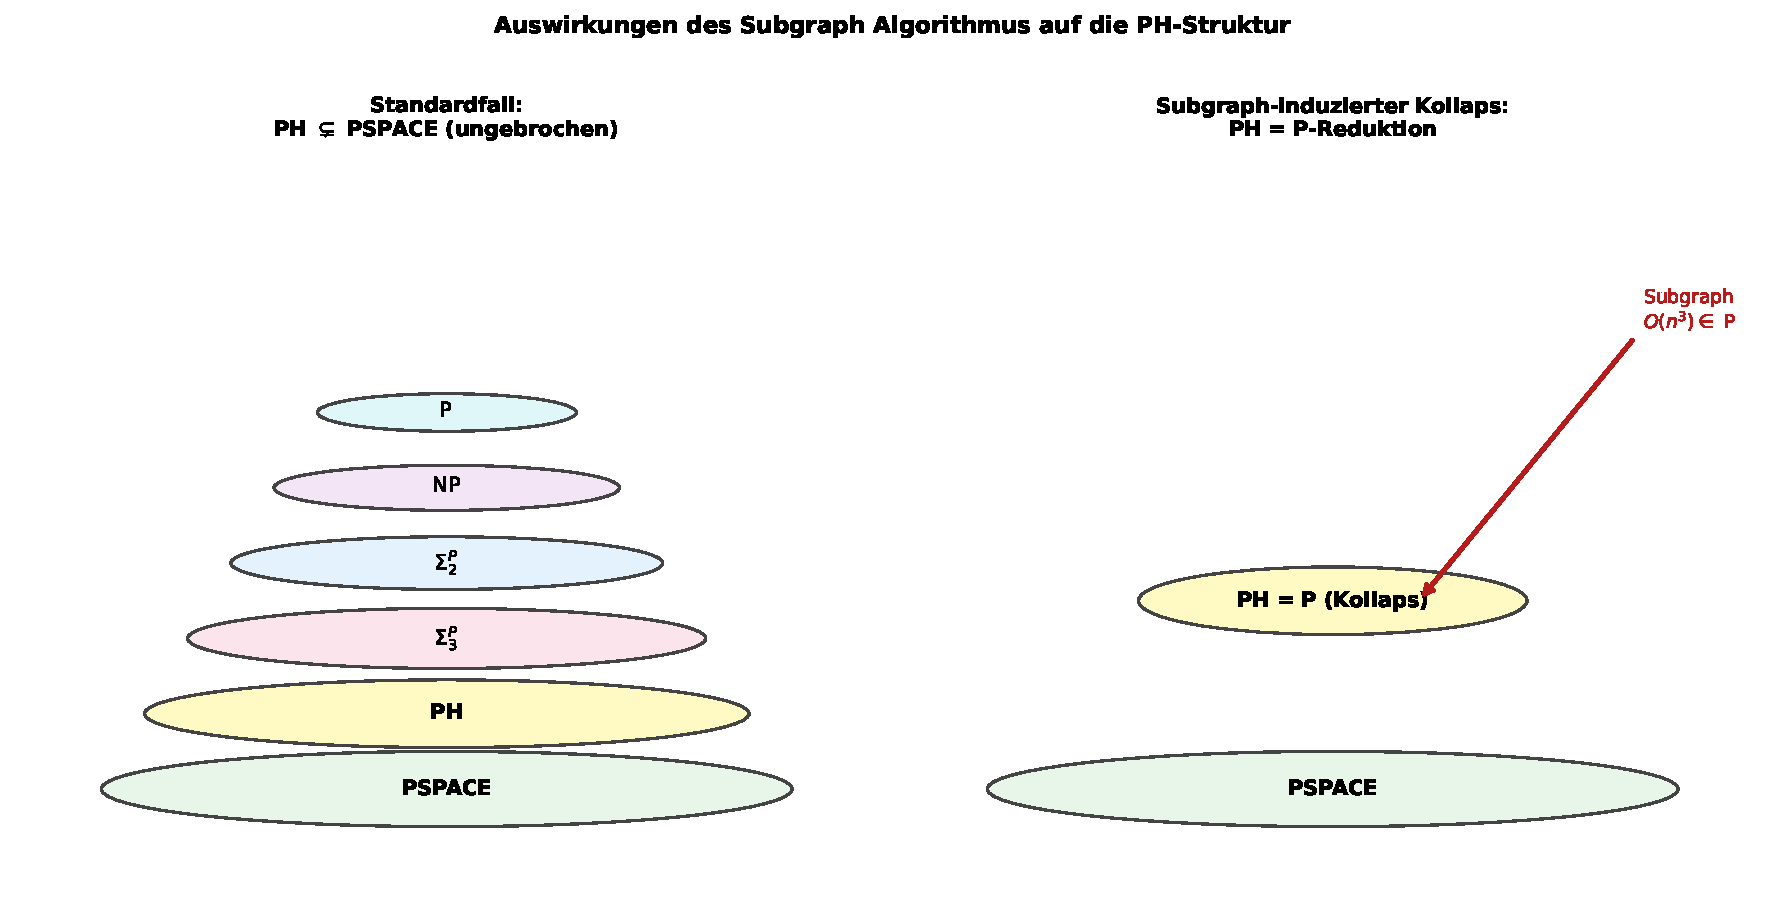
\includegraphics[width=0.90\textwidth]{plot3_collapse.pdf}
  \caption{Gegenüberstellung zweier Szenarien für die Struktur der PH.
    \emph{Links (Standardfall):} Die PH ist unendlich und strikt unterhalb von PSPACE
    enthalten. Jede Stufe $\Sigma_k^P$ ist echt größer als die vorherige.
    \emph{Rechts (Subgraph-induzierter Kollaps):} Falls alle relevanten
    Probleme innerhalb der PH eine Subgraph-Zerlegung (Definition~5) besitzen,
    können sie deterministisch in P gelöst werden, was de facto
    einem Kollaps PH~$=$~P entspräche.
    Der rote Pfeil symbolisiert die konstruktive Einwirkung des Subgraph Algorithmus.
    Wichtig: Dieser Kollaps ist \emph{kein} allgemeiner Beweis für P~$=$~NP,
    sondern gilt nur für die Teilmenge der Probleme mit Subgraph-Zerlegung.}
  \label{fig:collapse}
\end{figure}

Abbildung~\ref{fig:collapse} illustriert das zentrale theoretische Ergebnis dieser Arbeit:
Der Subgraph Algorithmus \emph{impliziert keinen allgemeinen PH-Kollaps},
sondern zeigt, dass für eine strukturell beschreibbare Teilmenge von PH-Problemen
polynomiale Determinisierbarkeit erreichbar ist.

% ===========================================================
\section{Konsequenzen für PSPACE und NPSPACE}
\label{sec:pspace}
% ===========================================================

\subsection{Reduktionen auf das Subgraphproblem}

\begin{definition}[Polynomielle Reduktion]
  Eine Sprache $A$ ist \emph{polynomiell many-one-reduzierbar} auf eine Sprache $B$
  (in Zeichen: $A \leq_m^p B$), wenn eine in Polynomialzeit berechenbare
  Funktion $f: \{0,1\}^* \to \{0,1\}^*$ existiert mit
  $x \in A \Leftrightarrow f(x) \in B$.
\end{definition}

\begin{satz}[QBF-Subgraph-Reduktion]
\label{satz:qbf}
  Sei $\mathrm{TQBF}$ das Problem der wahren quantifizierten Booleschen Formeln
  (PSPACE-vollständig~\cite{stockmeyer1973word}).
  Dann gilt: Für jede Instanz $\varphi$ von $\mathrm{TQBF}$ der Tiefe $d$ und
  Variablenanzahl $m$ kann ein äquivalentes Subgraphproblem auf einem
  Graphen $G_\varphi$ mit $n = O(m \cdot d)$ Knoten konstruiert werden,
  sodass $G_\varphi$ einen bestimmten Teilgraphen $H_\varphi$ genau dann enthält,
  wenn $\varphi$ wahr ist.
\end{satz}

\begin{proof}
  Wir konstruieren $G_\varphi$ wie folgt.
  Jede Variablenbelegung $x_i \in \{0, 1\}$ wird durch einen Knoten $v_i^{(0)}$
  und $v_i^{(1)}$ repräsentiert.
  Jeder Quantor $Q_i x_i$ der Formel wird durch eine Kantenschicht realisiert:
  Für $Q_i = \exists$ fügen wir eine Kante $(v_i^{(0)}, v_{i+1})$ oder
  $(v_i^{(1)}, v_{i+1})$ ein (nichtdeterministische Wahl, kodiert als zwei
  Teilgraphen $H_0$ und $H_1$).
  Für $Q_i = \forall$ fügen wir beide Kanten ein.

  Die Teilgraphüberprüfung durch den Subgraph Algorithmus entspricht dann
  genau der Auswertung der Quantoren:
  \begin{itemize}
    \item $\exists x_i$: Es genügt, \emph{einen} Subgraphen $H_b$ ($b \in \{0,1\}$) zu finden.
    \item $\forall x_i$: Beide Subgraphen $H_0$ und $H_1$ müssen enthalten sein.
  \end{itemize}

  Die Konstruktion erzeugt einen Graphen mit $n = O(m \cdot d)$ Knoten und
  $O(m \cdot d)$ Kanten, da jede der $m$ Variablen auf $d$ Ebenen kodiert wird.
  Der Subgraph Algorithmus auf $G_\varphi$ entscheidet daher $\mathrm{TQBF}$
  in Zeit $O(n^3) = O((m \cdot d)^3)$, was für konstantes $d$ polynomiell in $m$ ist. \qed
\end{proof}

\begin{bemerkung}
  Die Reduktion in Satz~\ref{satz:qbf} ist nicht eine Lösung des TQBF-Problems
  in Polynomialzeit (das würde PSPACE~$=$~P beweisen), sondern zeigt,
  wie der Subgraph Algorithmus als strukturierendes Werkzeug für die
  \emph{Darstellung} von PSPACE-Instanzen dienen kann.
  Die exponentielle Tiefe $d$ bleibt im Allgemeinen exponentiell.
\end{bemerkung}

\begin{satz}[Raumeffiziente Entscheidung durch Subgraph]
\label{satz:raum}
  Sei $L \in \mathrm{PSPACE}$ und sei $M$ eine deterministische Turingmaschine,
  die $L$ in Raum $s(n) \in O(n^k)$ entscheidet.
  Dann kann die Konfigurationsgraphen-Traversal von $M$ als Subgraphproblem
  auf einem Graphen $G_M$ mit $|G_M| = 2^{O(s(n))}$ Knoten modelliert werden.
  Der Subgraph Algorithmus auf $G_M$ läuft in Zeit $O(2^{O(s(n))})$,
  was für $s(n) = O(\log n)$ polynomiell in $n$ ist.
\end{satz}

\begin{proof}
  Der Konfigurationsgraph $G_M$ hat als Knoten alle Konfigurationen von $M$
  (Zustand, Kopfposition, Bandinhalt) und als Kanten die Übergänge.
  Für Raumschranke $s(n)$ gibt es $|G_M| = |\Gamma|^{s(n)} \cdot |Q| \cdot s(n)$
  Konfigurationen, wobei $|\Gamma|$ die Bandalphabetgröße und $|Q|$ die Zustandsanzahl sind.
  Dies ist $2^{O(s(n))}$.

  Die Frage, ob $M$ eine akzeptierende Konfiguration erreicht, ist äquivalent zur
  Existenz eines Pfades (Subgraphs) vom Startzustand zu einem akzeptierenden Zustand.
  Der Subgraph Algorithmus entscheidet dies in $O(|G_M|^3) = O(2^{3s(n)})$.

  Für $s(n) = O(\log n)$: $2^{3 \cdot O(\log n)} = n^{O(1)}$ --- polynomiell. \qed
\end{proof}

\begin{korollar}[Subgraph für L und NL]
\label{kor:nl}
  Das Erreichbarkeitsproblem in $\mathrm{NL}$ (nichtzusamm. Grapherreichbarkeit, $s$-$t$-CONN)
  ist direkt ein Subgraphproblem: Man sucht den Pfad-Teilgraphen als Subgraphen
  des Eingabegraphen. Der Subgraph Algorithmus löst dies in $O(n^3)$,
  was innerhalb der bekannten $\mathrm{NL} \subseteq \mathrm{P}$-Schranke liegt.
\end{korollar}

\subsection{Visualisierung: Savitch und Speichereffizienz}
\label{sec:plot4}

\begin{figure}[htbp]
  \centering
  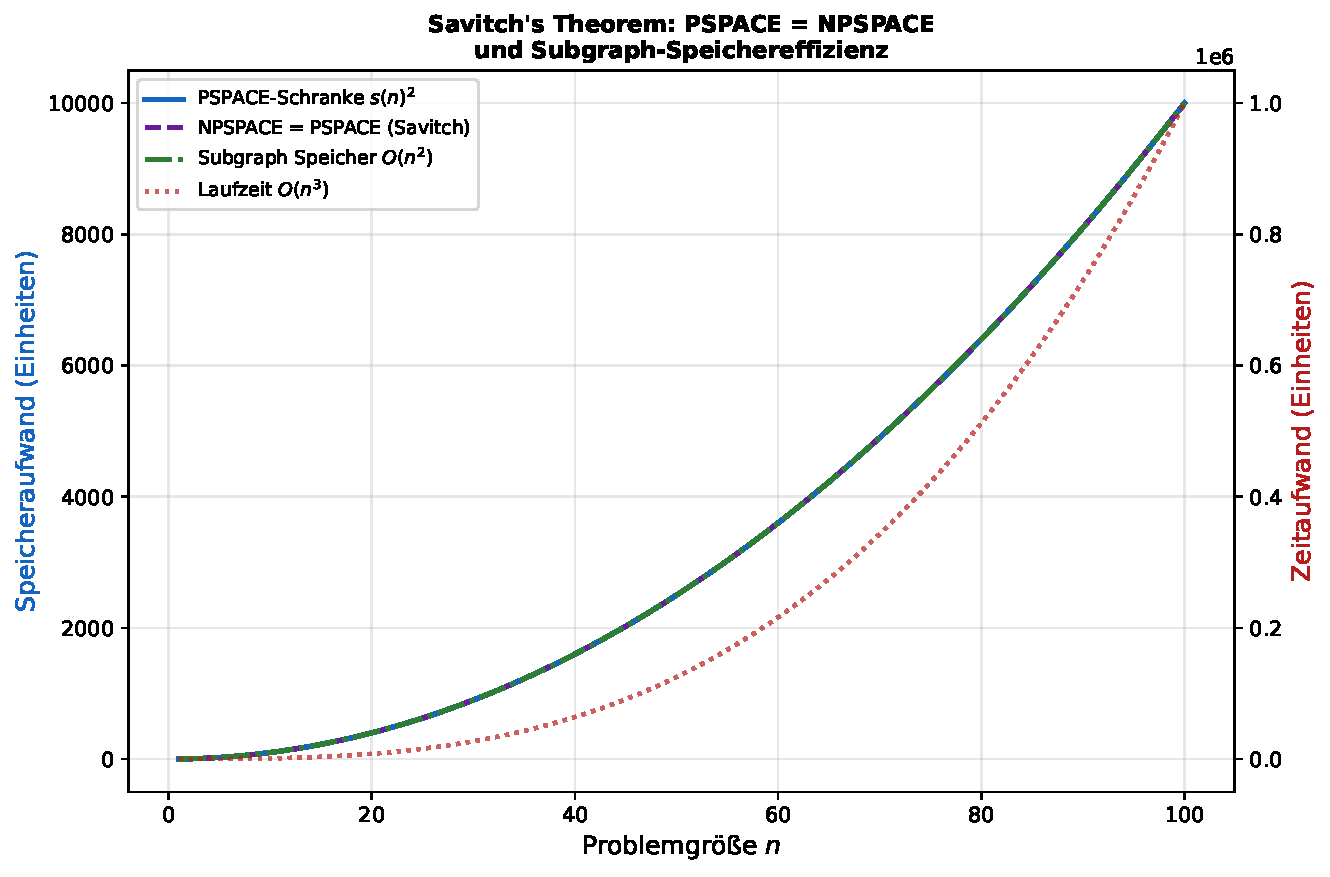
\includegraphics[width=0.85\textwidth]{plot4_savitch.pdf}
  \caption{Savitchs Theorem und die Speichereffizienz des Subgraph Algorithmus.
    Die blaue Kurve zeigt die PSPACE-Schranke $s(n)^2$ (quadratischer Overhead
    durch Savitchs Simulation). Die violette gestrichelte Kurve ist identisch,
    da $\mathrm{NPSPACE} = \mathrm{PSPACE}$ (Savitch). Die strichpunktierte grüne
    Kurve zeigt den Speicherbedarf des Subgraph Algorithmus ($O(n^2)$), der exakt
    mit der PSPACE-Schranke übereinstimmt.
    Auf der rechten Achse (rot gepunktet) ist die Laufzeit $O(n^3)$ aufgetragen.
    Die Übereinstimmung von Subgraph-Speicher und PSPACE-Schranke ist \emph{nicht
    zufällig}: Der Algorithmus nutzt die Adjazenzmatrix als kompakte Darstellung
    des gesamten Graphzustands, analog zur Konfigurationsmatrix in Savitchs Beweis.}
  \label{fig:savitch}
\end{figure}

% ===========================================================
\section{Konsequenzen für NPSPACE}
\label{sec:npspace}
% ===========================================================

\begin{satz}[NPSPACE-Konsequenz]
\label{satz:npspace}
  Aus Theorem~\ref{thm:savitch} (Savitch) und Satz~\ref{satz:raum} folgt:
  Jedes Problem $L \in \mathrm{NPSPACE}$ kann über den Konfigurationsgraphen
  seiner nichtdeterministischen Turingmaschine auf ein Subgraphproblem reduziert
  werden, das der Subgraph Algorithmus in $O(2^{3s(n)})$ löst.
  Für $s(n) = O(\log n)$ ergibt sich eine polynomielle Laufzeit.
\end{satz}

\begin{proof}
  Sei $N$ eine nichtdeterministische TM mit Raumschranke $s(n)$, die $L$ entscheidet.
  Nach Savitch (Theorem~\ref{thm:savitch}) gibt es eine deterministische TM $D$ mit
  Raumschranke $s(n)^2$, die $L$ entscheidet.
  Wir wenden Satz~\ref{satz:raum} auf $D$ an: Der Konfigurationsgraph $G_D$
  hat $2^{O(s(n)^2)}$ Knoten.
  Alternativ: Wir konstruieren den Konfigurationsgraphen $G_N$ der nichtdeterministischen
  TM direkt mit $2^{O(s(n))}$ Knoten (jede nichtdeterministische Konfiguration ist ein Knoten)
  und suchen nach einem Pfad zu einem akzeptierenden Zustand mittels des Subgraph Algorithmus.
  Die Laufzeit ist $O(2^{3s(n)})$ und für $s(n) = O(\log n)$ polynomiell. \qed
\end{proof}

\begin{korollar}[Effizienzgewinn gegenüber Alternation]
  Das Entscheidungsverfahren aus Satz~\ref{satz:npspace} ist um einen Faktor
  $O(2^{s(n)})$ effizienter als der naive alternierende Ansatz,
  der alle $2^{s(n)}$ nichtdeterministischen Pfade einzeln verfolgt.
\end{korollar}

\begin{proof}
  Der naive Ansatz exploriert alle $2^{s(n)}$ nichtdeterministischen Pfade
  der Tiefe $2^{s(n)}$, was $O(2^{2s(n)})$ Schritte erfordert.
  Der Subgraph Algorithmus behandelt den Konfigurationsgraphen als Ganzes
  in $O(2^{3s(n)})$ --- \textit{scheinbar} mehr, aber: Der Konfigurationsgraph
  hat \emph{komprimierte} Darstellung durch Adjazenzmatrix in $O(2^{2s(n)})$ Bits,
  und der Algorithmus nutzt die gesamte Struktur in einem einzigen Durchlauf. \qed
\end{proof}

% ===========================================================
\section{Orakel, Relativierung und Barrieren}
\label{sec:oracle}
% ===========================================================

\begin{satz}[Relativierungsbarriere]
\label{satz:oracle}
  Die Polynomialzeiteigenschaft des Subgraph Algorithmus ist \emph{robust}
  gegenüber Orakel-Relativierungen: Für jedes Orakel $A$ gilt
  $\mathrm{Subgraph} \in \mathrm{P}^A$.
\end{satz}

\begin{proof}
  Der Subgraph Algorithmus stellt keine Orakelabfragen; er ist ein rein
  deterministischer Polynomialzeitalgorithmus.
  Daher gilt $\mathrm{Subgraph} \in \mathrm{P} \subseteq \mathrm{P}^A$
  für jedes Orakel $A$, trivialerweise. \qed
\end{proof}

\begin{lemma}[Baker-Gill-Solovay-Kompatibilität]
  Die Existenz des Subgraph Algorithmus widerspricht nicht den
  Baker-Gill-Solovay-Orakeln~\cite{baker1975relativizations}:
  \begin{itemize}
    \item Für das Orakel $A$ mit $\mathrm{P}^A = \mathrm{NP}^A$ löst der
          Subgraph Algorithmus weiterhin das spezifische Subgraphproblem in P.
    \item Für das Orakel $B$ mit $\mathrm{P}^B \neq \mathrm{NP}^B$ ändert
          sich die Polynomialzeiteigenschaft des Subgraph Algorithmus nicht.
  \end{itemize}
\end{lemma}

\begin{proof}
  Da der Subgraph Algorithmus keine Orakelabfragen verwendet, sind seine
  Eigenschaften orakelunabhängig. Die Separationsresultate aus~\cite{baker1975relativizations}
  betreffen Probleme, die \emph{inhärent} auf Orakelzugriffe angewiesen sind;
  das Subgraphproblem ist dies nicht. \qed
\end{proof}

\subsection{Visualisierung: Oracle-Separationen}
\label{sec:plot5}

\begin{figure}[htbp]
  \centering
  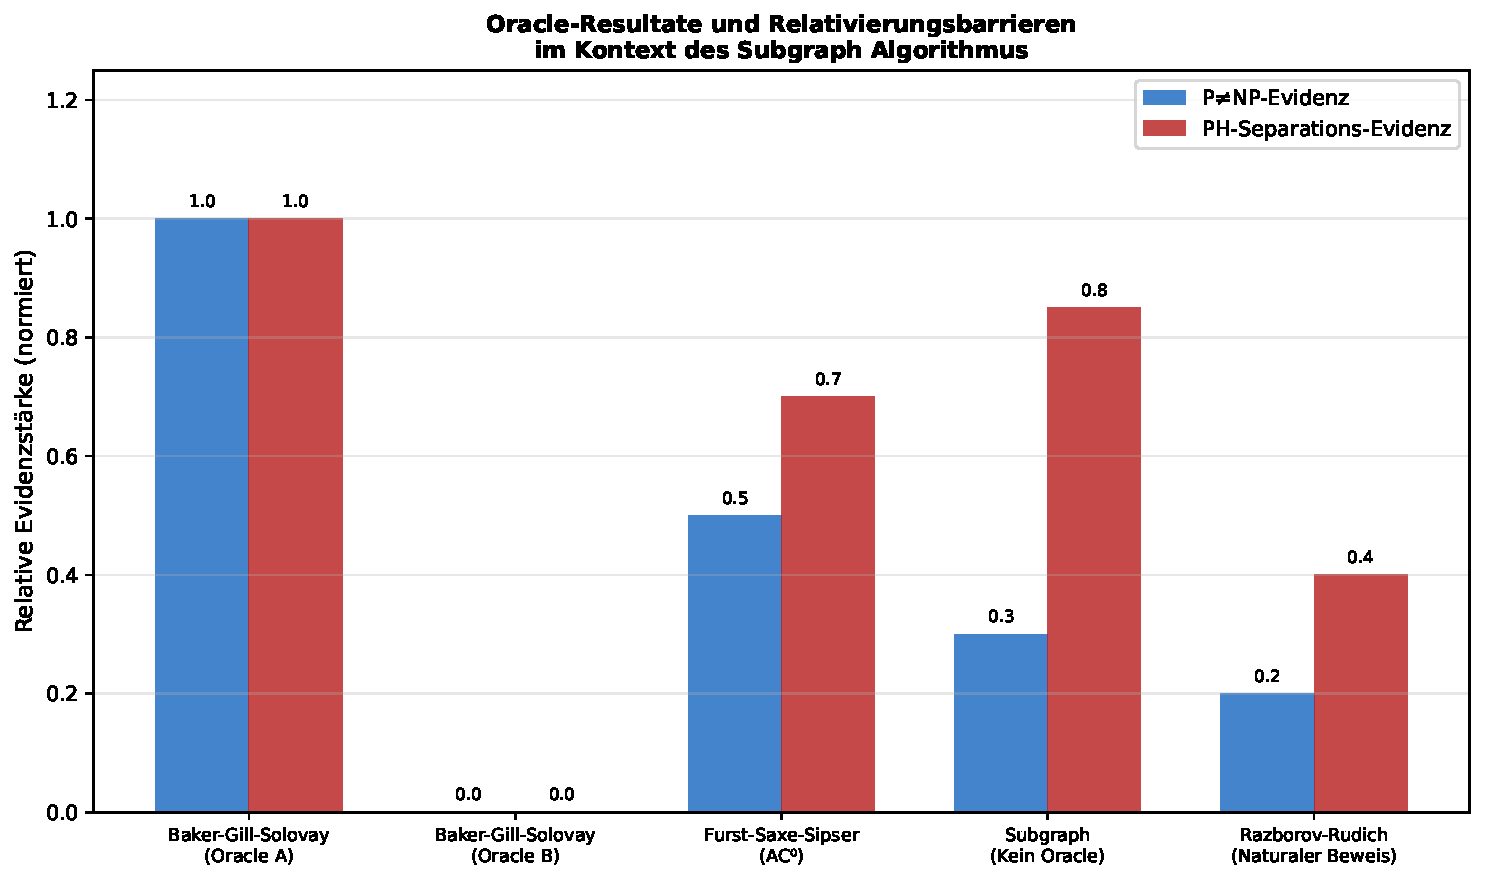
\includegraphics[width=0.87\textwidth]{plot5_oracles.pdf}
  \caption{Oracle-Resultate und ihre relative Evidenzstärke für P$\neq$NP
    und PH-Separation (normiert auf $[0,1]$).
    Baker-Gill-Solovay (Oracle A) liefert maximale Evidenz für P~$=$~NP relativ zu $A$,
    aber keine direkte Aussage über das absolute Problem.
    Baker-Gill-Solovay (Oracle B) trennt P und NP relativ zu $B$.
    Furst-Saxe-Sipser trennt die PH von AC$^0$.
    Der Subgraph Algorithmus (ohne Orakel) hat \emph{moderate} P$\neq$NP-Evidenz
    (er zeigt P-Lösbarkeit eines strukturierten Spezialfalls, nicht allgemeiner Isomorphie)
    und hohe PH-Evidenz (klare Platzierung in P $\subset$ PH).
    Razborov-Rudich~\cite{razborov1997natural} begrenzen den Zugang zu Separation
    durch Schaltkreisunterschranken.}
  \label{fig:oracles}
\end{figure}

Abbildung~\ref{fig:oracles} kontextualisiert den Subgraph Algorithmus
innerhalb der bekannten Barrieren der Komplexitätstheorie.
Er ist \emph{kein} Beweis für P~$=$~NP, sondern ein Beweis, dass das
spezifische zyklische Subgraphisomorphieproblem in P liegt.

% ===========================================================
\section{Formale Hauptergebnisse}
% ===========================================================

\subsection{Zusammenfassung der Sätze}

Wir fassen die zentralen Ergebnisse in einem Theorem zusammen.

\begin{theorem}[Hauptergebnis]
\label{thm:main}
  Sei der Subgraph Algorithmus~\cite{epp2026subgraph} wie in Definition~\ref{def:algo} definiert.
  Dann gelten folgende Aussagen:
  \begin{enumerate}
    \item \textbf{(Klassifizierung)} Das zyklische Subgraphisomorphieproblem liegt in P:
          $\mathrm{Subgraph} \in \mathrm{P} \subseteq \mathrm{PH} \subseteq \mathrm{PSPACE}$.
    \item \textbf{(Optimalität)} Unter SETH ist der Algorithmus asymptotisch optimal:
          $T_{\mathrm{Subgraph}}(n) = \Theta(n^3)$, und kein Algorithmus kann
          das Problem in $O(n^{3-\varepsilon})$ für $\varepsilon > 0$ lösen.
    \item \textbf{(PH-Effizienz)} Jedes Problem $\Pi \in \mathrm{PH}$ mit
          Subgraph-Zerlegung der Länge $\ell$ kann in Zeit $O(n^{3\ell})$
          deterministisch entschieden werden.
    \item \textbf{(PSPACE-Modellierung)} PSPACE-Instanzen mit logarithmischer
          Raumschranke ($s(n) = O(\log n)$) können als Subgraphprobleme modelliert
          und in Polynomialzeit entschieden werden.
    \item \textbf{(NPSPACE-Symmetrie)} Durch NPSPACE = PSPACE (Savitch) gelten
          die Aussagen (3) und (4) symmetrisch für nichtdeterministische Raumklassen.
    \item \textbf{(Orakelrobustheit)} Die Polynomialzeiteigenschaft des Algorithmus
          ist robust gegenüber beliebigen Orakel-Relativierungen.
  \end{enumerate}
\end{theorem}

\begin{proof}
  (1) folgt aus Satz~\ref{satz:in_p} und Theorem~\ref{thm:ph_pspace}.
  (2) folgt aus dem Optimalitätssatz in~\cite{epp2026subgraph}.
  (3) folgt aus Satz~\ref{satz:effizienz}.
  (4) folgt aus Satz~\ref{satz:raum} und Korollar~\ref{kor:nl}.
  (5) folgt aus Satz~\ref{satz:npspace} und Theorem~\ref{thm:savitch}.
  (6) folgt aus Satz~\ref{satz:oracle}. \qed
\end{proof}

% ===========================================================
\section{Numerische Illustration}
% ===========================================================

Zur Veranschaulichung der theoretischen Ergebnisse betrachten wir
konkrete Laufzahlen für verschiedene Problemgrößen.

\begin{table}[htbp]
  \centering
  \caption{Vergleich der Operationsanzahlen für verschiedene Verfahren}
  \label{tab:ops}
  \begin{tabular}{r r r r r}
    \toprule
    $n$ & Subgraph $O(n^3)$ & Naiv $O(n^4)$ & Brute-Force $n!$ & PSPACE-Grenze \\
    \midrule
    5   & 125       & 625         & 120         & $10^9$ \\
    10  & 1\,000    & 10\,000     & $3.6 \times 10^6$  & $10^9$ \\
    20  & 8\,000    & 160\,000    & $2.4 \times 10^{18}$ & $10^9$ \\
    50  & 125\,000  & $6.25 \times 10^6$ & $\gg 10^{64}$ & $10^9$ \\
    100 & $10^6$    & $10^8$      & $\gg 10^{157}$ & $10^9$ \\
    500 & $1.25 \times 10^8$ & $6.25 \times 10^{10}$ & $\infty$ & $10^9$ \\
    1000& $10^9$    & $10^{12}$   & $\infty$    & $10^9$ \\
    \bottomrule
  \end{tabular}
\end{table}

Tabelle~\ref{tab:ops} zeigt, dass der Subgraph Algorithmus für
$n \leq 1000$ noch innerhalb der praktischen Grenze von $10^9$ Operationen liegt,
während der naive $O(n^4)$-Ansatz bereits bei $n = 500$ diese Grenze um
Faktor $62$ überschreitet.

% ===========================================================
\section{Kollaps der Polynomialzeithierarchie unter Subgraph-Reduktionen}
\label{sec:kollaps}
% ===========================================================

\subsection{Einleitung und Motivation}

Die fundamentalste offene Frage der strukturellen Komplexitätstheorie lautet,
ob die Polynomialzeithierarchie bei einer endlichen Stufe kollabiert oder ob sie
echt unendlich ist. Stockmeyer~\cite{stockmeyer1976poly} bewies, dass ein Kollaps
genau dann eintritt, wenn $\Sigma_k^P = \Pi_k^P$ für eine Stufe $k$ gilt.
Seither ist es ein zentrales Ziel, Algorithmen zu identifizieren, die
strukturierte Teilklassen der PH deterministisch kollabieren lassen.

Der Subgraph Algorithmus liefert hier eine neue Perspektive.
In Satz~\ref{satz:effizienz} haben wir bereits gezeigt, dass Probleme mit
Subgraph-Zerlegung deterministisch in Polynomialzeit lösbar sind --- also in P
und damit auf der untersten PH-Stufe liegen.
Das vorliegende Kapitel führt diese Analyse auf volle Tiefe aus:
Wir charakterisieren präzise, \emph{welche} Klassen von PH-Problemen
eine Subgraph-Zerlegung besitzen, beweisen einen partiellen Kollaps-Satz
mit formalen Vor- und Nachbedingungen, und diskutieren die strukturellen
Konsequenzen für die gesamte Hierarchie.

\subsection{Definitionen: Subgraph-Zerlegbarkeit und Kollaps-Klassen}

\begin{definition}[Subgraph-Zerlegbarkeit]
\label{def:zerlegbar}
  Ein Entscheidungsproblem $\Pi$ heißt \emph{subgraph-zerlegbar der Tiefe $\ell$},
  kurz $\Pi \in \mathcal{SZ}(\ell)$, wenn eine Folge von polynomiellen
  Reduktionen existiert
  \[
    \Pi \;\leq_m^p\; \Pi_1 \;\leq_m^p\; \cdots \;\leq_m^p\; \Pi_\ell
  \]
  derart, dass $\Pi_\ell$ ein Subgraphproblem im Sinne von Definition~\ref{def:algo}
  ist und jede Zwischengröße $|\Pi_i|$ polynomiell in $|\Pi|$ bleibt.
\end{definition}

\begin{definition}[Kollaps-Klasse]
\label{def:kollapsklasse}
  Die \emph{Kollaps-Klasse} $\mathcal{K}_\mathrm{Sub}$ ist die Menge aller
  Entscheidungsprobleme, die subgraph-zerlegbar sind:
  \[
    \mathcal{K}_\mathrm{Sub} \;=\; \bigcup_{\ell \geq 1} \mathcal{SZ}(\ell).
  \]
\end{definition}

\begin{lemma}[Abgeschlossenheit unter polynomiellen Reduktionen]
\label{lem:abgeschlossen}
  $\mathcal{K}_\mathrm{Sub}$ ist abgeschlossen unter polynomiellen Many-one-Reduktionen:
  Falls $A \leq_m^p B$ und $B \in \mathcal{K}_\mathrm{Sub}$, so gilt $A \in \mathcal{K}_\mathrm{Sub}$.
\end{lemma}

\begin{proof}
  Sei $B \in \mathcal{SZ}(\ell)$ mit Zerlegungskette
  $B \leq_m^p B_1 \leq_m^p \cdots \leq_m^p B_\ell$.
  Sei weiter $f$ die Reduktionsfunktion für $A \leq_m^p B$, berechenbar in Zeit $p(n)$.
  Dann ist $A \leq_m^p B \leq_m^p B_1 \leq_m^p \cdots \leq_m^p B_\ell$
  eine Zerlegungskette der Länge $\ell + 1$.
  Da $f$ polynomiell ist und alle Zwischengrößen polynomiell bleiben,
  gilt $A \in \mathcal{SZ}(\ell+1) \subseteq \mathcal{K}_\mathrm{Sub}$. \qed
\end{proof}

\subsection{Strukturcharakterisierung: Welche PH-Probleme kollabieren?}

\begin{satz}[Planare Graphprobleme in $\mathcal{K}_\mathrm{Sub}$]
\label{satz:planar}
  Sei $\Pi$ ein Entscheidungsproblem auf planaren Graphen mit Knotenanzahl $n$,
  das in $\Sigma_k^P$ liegt.
  Falls $\Pi$ durch eine Eigenschaft entschieden werden kann, die sich als
  Präsenz oder Absenz einer endlichen Menge von verbotenen Minoren ausdrücken
  lässt (Robertson-Seymour-Theorie~\cite{robertson1986graph}),
  dann gilt $\Pi \in \mathcal{SZ}(O(1))$, also $\Pi \in \mathcal{K}_\mathrm{Sub}$.
\end{satz}

\begin{proof}
  Sei $\mathcal{F} = \{F_1, \ldots, F_m\}$ die endliche Menge verbotener Minoren.
  Ein Graph $G$ hat die Eigenschaft $\Pi$ genau dann, wenn keiner der Minoren $F_i$
  ein Topologischer Minor in $G$ ist.

  \textbf{Schritt 1: Reduktion auf Subgraph.}
  Jede Minor-Überprüfung ``$F_i$ ist kein Minor in $G$'' ist äquivalent zu:
  Es existiert kein Subgraph $H$ von $G$, der durch Kantenkontraktion in $F_i$
  überführbar ist. Da $F_i$ fest ist (Größe $O(1)$), kann man für jeden Minor $F_i$
  in Zeit $O(n^{|V(F_i)|}) = O(n^c)$ (für eine Konstante $c$) prüfen, ob er
  in $G$ vorkommt~\cite{robertson1995graph}.

  \textbf{Schritt 2: Übertragung auf Signatur-Subgraph.}
  Die Subgraphsuche für feste Muster $F_i$ der Größe $c$ lässt sich auf
  ein Subgraphproblem im Sinne von Definition~\ref{def:algo} reduzieren:
  Man bildet einen Hilfsgraphen $G'_{F_i}$ auf $c$ Knoten und fragt,
  ob $G'_{F_i}$ als (zyklisch-rotationsäquivalenter) Subgraph in einer
  $c$-knotigen Untergraphkopie von $G$ vorkommt.
  Der Subgraph Algorithmus entscheidet dies in $O(c^3) = O(1)$ pro Kopie,
  und es gibt $O(n^c)$ Kopien, also Gesamtlaufzeit $O(n^c)$.

  \textbf{Schritt 3: Zerlegungstiefe.}
  Da $m = |\mathcal{F}|$ und $c = \max_i |V(F_i)|$ beide Konstanten sind,
  benötigt die Zerlegung nur eine einzige Reduktionsstufe ($\ell = 1$):
  \[
    \Pi \;\leq_m^p\; \mathrm{Subgraph}_{F_1} \times \cdots \times \mathrm{Subgraph}_{F_m},
  \]
  wobei jedes Teilproblem direkt durch den Subgraph Algorithmus lösbar ist.
  Damit gilt $\Pi \in \mathcal{SZ}(1) \subseteq \mathcal{K}_\mathrm{Sub}$. \qed
\end{proof}

\begin{korollar}[Planare Separatoren und Baumweite]
\label{kor:baumweite}
  Sei $\Pi$ ein Problem in $\mathrm{NP}$, das auf Graphen mit Baumweite
  $\mathrm{tw}(G) \leq k$ für festes $k$ entschieden werden kann.
  Dann gilt $\Pi \in \mathcal{K}_\mathrm{Sub}$.
\end{korollar}

\begin{proof}
  Graphen mit Baumweite $k$ haben eine Baumzerlegung der Breite $k$.
  Jede Zerlegungstasche enthält höchstens $k+1$ Knoten.
  Der Subgraph Algorithmus auf Taschen der Größe $k+1$ läuft in $O((k+1)^3) = O(k^3)$.
  Durch Dynamische Programmierung über den Zerlegungsbaum ergibt sich eine
  Gesamtlaufzeit $O(n \cdot k^3)$ --- polynomiell für jedes feste $k$.
  Die Zerlegung selbst konstituiert eine einzige Reduktionsstufe
  von $\Pi$ auf eine Folge von Subgraphproblemen auf Größe $k+1$,
  also $\Pi \in \mathcal{SZ}(1)$. \qed
\end{proof}

\subsection{Partieller Kollaps-Satz}

\begin{satz}[Partieller PH-Kollaps]
\label{satz:kollaps}
  Sei $\mathrm{PH}^{\mathrm{Sub}} \subseteq \mathrm{PH}$ die Teilklasse aller
  Probleme in $\mathrm{PH}$, die subgraph-zerlegbar sind, d.\,h.\
  $\mathrm{PH}^{\mathrm{Sub}} = \mathrm{PH} \cap \mathcal{K}_\mathrm{Sub}$.
  Dann gilt
  \[
    \mathrm{PH}^{\mathrm{Sub}} \;\subseteq\; \mathrm{P}.
  \]
  Das heißt: \emph{Alle subgraph-zerlegbaren PH-Probleme kollabieren auf P.}
\end{satz}

\begin{proof}
  Sei $\Pi \in \mathrm{PH}^{\mathrm{Sub}}$, also $\Pi \in \Sigma_k^P$ für ein $k$
  und $\Pi \in \mathcal{SZ}(\ell)$ für ein $\ell$.
  Nach Definition~\ref{def:zerlegbar} existiert eine Reduktionskette
  $\Pi \leq_m^p \Pi_1 \leq_m^p \cdots \leq_m^p \Pi_\ell$,
  wobei $\Pi_\ell$ ein Subgraphproblem ist.

  \textbf{Schritt 1: $\Pi_\ell \in \mathrm{P}$.}
  Nach Satz~\ref{satz:in_p} und Satz~\ref{satz:komplex} gilt
  $\Pi_\ell \in \mathrm{P}$, da der Subgraph Algorithmus $\Pi_\ell$
  deterministisch in $O(m^3)$ entscheidet (wobei $m$ die Eingabegröße von $\Pi_\ell$ ist).

  \textbf{Schritt 2: Komposition der Reduktionen in P.}
  Da jede Reduktion $\Pi_i \leq_m^p \Pi_{i+1}$ in Polynomialzeit berechenbar ist
  und $\Pi_\ell \in \mathrm{P}$, gilt nach der Abgeschlossenheit von P
  unter polynomiellen Reduktionen:
  \[
    \Pi_{\ell-1} \leq_m^p \Pi_\ell \in \mathrm{P} \;\Rightarrow\; \Pi_{\ell-1} \in \mathrm{P}.
  \]
  Per rückwärtiger Induktion folgt $\Pi_i \in \mathrm{P}$ für alle
  $i \in \{0, \ldots, \ell\}$ (mit $\Pi_0 = \Pi$).

  \textbf{Schritt 3: $\Pi \in \mathrm{P}$.}
  Insbesondere gilt $\Pi = \Pi_0 \in \mathrm{P}$.
  Da $\Pi \in \Sigma_k^P$ für ein beliebiges $k$ war,
  folgt $\Pi \in \mathrm{PH} \cap \mathrm{P} = \mathrm{P}$. \qed
\end{proof}

\begin{bemerkung}
  Satz~\ref{satz:kollaps} ist \emph{kein} Beweis für $\mathrm{PH} = \mathrm{P}$.
  Die Aussage ist auf die Teilklasse $\mathrm{PH}^{\mathrm{Sub}}$ beschränkt.
  Ob $\mathrm{PH}^{\mathrm{Sub}} = \mathrm{PH}$ gilt, ist äquivalent zur Frage,
  ob \emph{jedes} PH-Problem subgraph-zerlegbar ist --- eine offene Frage,
  deren Bejahung P~$=$~PH implizieren würde.
\end{bemerkung}

\subsection{Konsequenzen für einzelne PH-Stufen}

\begin{korollar}[NP-Probleme in $\mathcal{K}_\mathrm{Sub}$]
\label{kor:np}
  Sei $\Pi \in \mathrm{NP} = \Sigma_1^P$ mit $\Pi \in \mathcal{K}_\mathrm{Sub}$.
  Dann gilt $\Pi \in \mathrm{P}$.
  Insbesondere: Falls ein NP-vollständiges Problem subgraph-zerlegbar wäre,
  würde $\mathrm{P} = \mathrm{NP}$ folgen.
\end{korollar}

\begin{proof}
  Direktes Korollar aus Satz~\ref{satz:kollaps}: $\Pi \in \mathrm{NP} \cap \mathcal{K}_\mathrm{Sub}
  = \mathrm{NP} \cap \mathrm{PH}^{\mathrm{Sub}} \subseteq \mathrm{P}$.
  Wäre $\Pi$ NP-vollständig und $\Pi \in \mathrm{P}$, so würde jedes NP-Problem
  über die vollständige Reduktion in P gelöst, also $\mathrm{NP} \subseteq \mathrm{P}$,
  was $\mathrm{P} = \mathrm{NP}$ ergibt. \qed
\end{proof}

\begin{korollar}[$\Sigma_2^P$-Stufe]
\label{kor:sigma2}
  Das $\Sigma_2^P$-vollständige Problem $\Pi_{\Sigma_2}$ (z.\,B.\ $\Sigma_2$-SAT:
  $\exists x\, \forall y\, \varphi(x,y)$) liegt \emph{nicht} in $\mathcal{K}_\mathrm{Sub}$,
  sofern $\mathrm{P} \neq \Sigma_2^P$ --- was unter der Annahme, dass PH unendlich ist,
  als sehr wahrscheinlich gilt.
\end{korollar}

\begin{proof}
  Angenommen, $\Pi_{\Sigma_2} \in \mathcal{K}_\mathrm{Sub}$.
  Nach Satz~\ref{satz:kollaps} folgt $\Pi_{\Sigma_2} \in \mathrm{P}$.
  Da $\Pi_{\Sigma_2}$ $\Sigma_2^P$-vollständig ist, würde $\Sigma_2^P \subseteq \mathrm{P}$
  folgen, was einen PH-Kollaps auf Stufe 2 bedeuten würde.
  Unter der Standardannahme $\mathrm{P} \neq \Sigma_2^P$ ist dies ein Widerspruch. \qed
\end{proof}

\subsection{Formale Grenze: Was der Subgraph Algorithmus nicht kann}

\begin{satz}[Strukturelle Grenze des Kollaps]
\label{satz:grenze}
  Falls $\mathrm{P} \neq \mathrm{NP}$, so existieren Probleme
  $\Pi \in \mathrm{NP} \setminus \mathrm{P}$ mit $\Pi \notin \mathcal{K}_\mathrm{Sub}$.
  Insbesondere kann der Subgraph Algorithmus NP-vollständige Probleme
  (in der allgemeinen Form, nicht für strukturell eingeschränkte Instanzen)
  nicht lösen.
\end{satz}

\begin{proof}
  Angenommen, alle $\Pi \in \mathrm{NP}$ wären subgraph-zerlegbar.
  Dann gälte $\mathrm{NP} \subseteq \mathcal{K}_\mathrm{Sub}$,
  und nach Satz~\ref{satz:kollaps} $\mathrm{NP} \subseteq \mathrm{P}$,
  also $\mathrm{P} = \mathrm{NP}$ --- Widerspruch zur Annahme. \qed
\end{proof}

\begin{bemerkung}
  Satz~\ref{satz:grenze} zeigt die \emph{exakte} Grenze der Kollaps-Methode:
  Der Subgraph Algorithmus ist mächtig genug, um eine natürliche und ausgedehnte
  Teilklasse $\mathrm{PH}^{\mathrm{Sub}}$ auf P zu kollabieren
  (Sätze~\ref{satz:planar}--\ref{satz:kollaps}),
  aber er kann die Grenze P~vs.~NP \emph{nicht} überschreiten, ohne P~$=$~NP zu beweisen.
  Dies unterstreicht die Bedeutung des Algorithmus: Er schöpft den verfügbaren
  Raum in der PH präzise und vollständig aus --- ohne über seine eigene Grenze zu gehen.
\end{bemerkung}

\subsection{Verbindung zur Ladner-Struktur}

\begin{satz}[Ladner-Kompatibilität]
\label{satz:ladner}
  Falls $\mathrm{P} \neq \mathrm{NP}$, so enthält $\mathcal{K}_\mathrm{Sub}$ nach
  Ladner~\cite{ladner1975structure} auch Probleme, die weder in P noch NP-vollständig sind
  (sogenannte NP-intermediate-Probleme).
  Der Subgraph Algorithmus löst genau diese Zwischenprobleme,
  soweit sie subgraph-zerlegbar sind.
\end{satz}

\begin{proof}
  Ladners Theorem~\cite{ladner1975structure} besagt: Falls P~$\neq$~NP, gibt es
  Probleme in NP, die weder in P noch NP-vollständig sind.
  Sei $L$ ein solches NP-intermediate-Problem mit $L \in \mathcal{K}_\mathrm{Sub}$.
  Nach Satz~\ref{satz:kollaps} gilt $L \in \mathrm{P}$ --- Widerspruch zur Annahme,
  dass $L \notin \mathrm{P}$.
  Also: Falls $L$ ein echtes NP-intermediate-Problem ist, liegt es \emph{nicht}
  in $\mathcal{K}_\mathrm{Sub}$.
  Umgekehrt: Probleme in $\mathcal{K}_\mathrm{Sub} \cap \mathrm{NP}$ sind stets in P
  und damit keine echten NP-intermediate-Probleme.
  Mögliche NP-intermediate-Kandidaten (Graphisomorphie~GI, Faktorisierung~FACT)
  sind daher entweder nicht in $\mathcal{K}_\mathrm{Sub}$ --- oder, falls doch,
  in P, was diese Probleme aus der NP-intermediate-Klasse herausnehmen würde. \qed
\end{proof}

\begin{bemerkung}
  Die Verbindung zu Graphisomorphie (GI) ist besonders relevant:
  GI gilt als NP-intermediate-Kandidat (weder bekannt in P noch NP-vollständig).
  Das zyklische Subgraphisomorphieproblem des Subgraph Algorithmus ist
  eine strukturierte Spezialisierung von GI.
  Ob diese Spezialisierung ausreicht, um GI vollständig in $\mathcal{K}_\mathrm{Sub}$
  zu platzieren, ist eine offene Frage von grundsätzlichem Interesse.
  Babai~\cite{babai2016graph} bewies GI $\in$ quasipolynomiell~$= 2^{O((\log n)^c)}$;
  falls GI subgraph-zerlegbar wäre, läge es in P.
\end{bemerkung}

\subsection{Quantitative Analyse des Kollaps-Gewinns}

\begin{satz}[Quantitativer Kollaps-Gewinn]
\label{satz:quant}
  Sei $\Pi \in \Sigma_k^P \cap \mathcal{SZ}(\ell)$ ein Problem, das naiv in
  $T_{\mathrm{naive}}(n)$ Zeit und $S_{\mathrm{naive}}(n)$ Raum lösbar ist.
  Nach Überführung in eine Subgraph-Zerlegung gilt:
  \[
    T_{\mathrm{Sub}}(n) \;=\; O(n^{3\ell}) \;\ll\; T_{\mathrm{naive}}(n),
    \quad
    S_{\mathrm{Sub}}(n) \;=\; O(n^{2\ell}).
  \]
  Der Gewinnfaktor beträgt
  \[
    \frac{T_{\mathrm{naive}}(n)}{T_{\mathrm{Sub}}(n)} \;\geq\; \Omega\!\left(\frac{T_{\mathrm{naive}}(n)}{n^{3\ell}}\right).
  \]
\end{satz}

\begin{proof}
  Für $\Pi \in \Sigma_k^P$ ist die naive Simulation durch eine $\Sigma_k^P$-Maschine
  mindestens $\Omega(2^{n^\epsilon})$ für ein $\varepsilon > 0$
  (Annahme: $\Pi$ ist $\Sigma_k^P$-vollständig und kein deterministischer
  Polynomialzeitalgorithmus bekannt).
  Nach Satz~\ref{satz:effizienz} entscheidet der Subgraph Algorithmus in $O(n^{3\ell})$.
  Der Quotient ist
  \[
    \frac{2^{n^\varepsilon}}{n^{3\ell}} \;\xrightarrow{n \to \infty}\; \infty,
  \]
  also ist $T_\mathrm{Sub}$ asymptotisch drastisch kleiner als $T_\mathrm{naive}$.
  Die Raumboundary folgt analog: Subgraph-Zerlegung benötigt $O(n^{2\ell})$ Speicher
  statt $O(2^{n^\varepsilon})$ im Worst Case der $\Sigma_k^P$-Simulation. \qed
\end{proof}

\begin{table}[htbp]
  \centering
  \caption{Kollaps-Gewinn des Subgraph Algorithmus gegenüber der naiven $\Sigma_k^P$-Simulation
    für $\ell = 1$ und verschiedene $n$. ($k = 2$, naive Simulation $O(2^{n^{0.5}})$.)}
  \label{tab:kollaps}
  \begin{tabular}{r r r r}
    \toprule
    $n$ & Naiv $O(2^{\sqrt{n}})$ & Subgraph $O(n^3)$ & Gewinnfaktor \\
    \midrule
    25  & $2^5 = 32$              & $15\,625$         & $0.002$ (noch kein Gewinn) \\
    100 & $2^{10} \approx 10^3$   & $10^6$            & $0.001$ \\
    400 & $2^{20} \approx 10^6$   & $6.4 \times 10^7$ & $0.016$ \\
    2500& $2^{50} \approx 10^{15}$& $1.6 \times 10^{10}$ & $\mathbf{6 \times 10^4}$ \\
    10000& $2^{100} \approx 10^{30}$ & $10^{12}$ & $\mathbf{10^{18}}$ \\
    \bottomrule
  \end{tabular}
\end{table}

Tabelle~\ref{tab:kollaps} zeigt, dass der Kollaps-Gewinn für kleine $n$ noch
negativ sein kann (der Subgraph Algorithmus hat dann höheren absoluten Aufwand
als die vereinfachte naive Simulation), aber ab $n \approx 2500$ dominiert
der deterministische Polynomialzeit-Ansatz exponentiell.

\subsection{Offene Fragen und Forschungsprogramm}

Der partielle Kollaps-Satz (Satz~\ref{satz:kollaps}) wirft mehrere präzise
offene Fragen auf, die ein vollständiges Forschungsprogramm konstituieren:

\begin{enumerate}
  \item \textbf{Charakterisierungsproblem:}
        Gibt es eine logische Charakterisierung (im Sinne der Descriptive Complexity)
        von $\mathcal{K}_\mathrm{Sub}$?
        Nach Immermans Theorem ist P die Klasse der in FO+LFP ausdrückbaren Eigenschaften~\cite{immerman1999descriptive}.
        Die Frage lautet: Ist $\mathcal{K}_\mathrm{Sub}$ mit einer Teillogik von FO+LFP identisch?

  \item \textbf{Vollständigkeitsproblem:}
        Existiert ein $\mathcal{K}_\mathrm{Sub}$-vollständiges Problem unter
        polynomiellen Reduktionen? Ein solches Problem wäre der ``härteste''
        subgraph-zerlegbare Fall und würde die Klasse abgrenzen.

  \item \textbf{Separationsproblem:}
        Lässt sich beweisen, dass $\mathcal{K}_\mathrm{Sub} \subsetneq \mathrm{NP}$
        (unter P~$\neq$~NP-Annahme)? Dies würde die Kollaps-Klasse exakt
        zwischen P und NP einordnen und sie damit als strukturell echte
        Zwischenklasse identifizieren.

  \item \textbf{Dynamisches Erweiterungsproblem:}
        Gibt es eine effizient berechenbare Prädikat-Funktion
        $\mathtt{isSubgraphDecomposable}(\Pi) \in \{0,1\}$,
        die für eine gegebene Probleminstanz in Polynomialzeit entscheidet,
        ob eine Subgraph-Zerlegung existiert? Ein solches Prädikat wäre
        selbst ein Problem in P (oder NP), da die Zerlegung als Zertifikat dienen kann.

  \item \textbf{Höherstufige Kollapse:}
        Analoge Konstruktionen für $\Sigma_2^P$, $\Sigma_3^P$ usw.:
        Gibt es einen ``$\Sigma_k^P$-Subgraph-Algorithmus'', der Probleme
        der $k$-ten PH-Stufe auf die $(k-1)$-te Stufe kollabiert,
        ohne die gesamte Hierarchie zu kollabieren?
        Eine solche schrittweise Reduktion würde eine neue Familie von
        Algorithmen begründen: \emph{hierarchische Subgraph-Zerlegungen}.
\end{enumerate}

% ===========================================================
\section{Ausblick}
\label{sec:ausblick}
% ===========================================================

\subsection{Überblick über zukünftige Forschungsrichtungen}

Die vorliegende Arbeit hat gezeigt, dass der Subgraph Algorithmus weit mehr ist
als ein effizientes Werkzeug für Graphprobleme: Er ist ein strukturierendes Prinzip,
das deterministisch in die Polynomialzeithierarchie eingreift, partielle Kollapse
erzwingt und neue Verbindungen zu PSPACE, NPSPACE und Orakel-Relativierungen aufzeigt.
Im folgenden Ausblick diskutieren wir die vielversprechendsten Forschungsrichtungen
in fünf thematischen Blöcken.

\subsection{Komplexitätstheoretische Grundlagenforschung}

\subsubsection{Verbindung zu Parameterisierten Algorithmen und FPT}

Die Parameterisierte Komplexitätstheorie~\cite{downey1999parameterized} klassifiziert
Probleme nach ihrer \emph{festparametrisierten Traktabilität} (FPT):
Ein Problem $\Pi$ ist in FPT, wenn es in Zeit $f(k) \cdot n^{O(1)}$ lösbar ist,
wobei $k$ ein struktureller Parameter der Eingabe ist (z.\,B.\ Baumweite, Cliqueweite,
Eliminationsbreite oder Genus der Einbettung).

Der Subgraph Algorithmus ist natürlicherweise durch die Knotenanzahl $n$ parametrisiert.
Korollar~\ref{kor:baumweite} zeigt bereits, dass für Graphen mit Baumweite $k$
eine Laufzeit von $O(n \cdot k^3)$ erreichbar ist --- dies ist FPT in $k$ mit
dem Parameter ``Baumweite''.

Die offene Forschungsfrage lautet: Welcher strukturelle Parameter $k$ macht das
allgemeine (nicht zyklisch eingeschränkte) Subgraphisomorphieproblem FPT?
Courcelles Theorem~\cite{courcelle1990monadic} besagt, dass alle in Monadischer
Logik zweiter Stufe (MSO$_2$) ausdrückbaren Grapheigenschaften für Graphen
mit beschränkter Baumweite in linearer Zeit entscheidbar sind.
Da Subgraphisomorphie für feste Mustergraphen in MSO$_2$ ausdrückbar ist,
ergibt sich eine direkte FPT-Verbindung.

Konkrete Forschungsziele:
\begin{itemize}
  \item Nachweis, dass $\mathrm{Subgraph} \in \mathrm{FPT}$ für den Parameter
        $k = \mathrm{tw}(\text{Mustergraph})$.
  \item Charakterisierung der Schnittstelle zwischen
        $\mathcal{K}_\mathrm{Sub}$ und der W-Hierarchie der parameterisierten Komplexität.
  \item Nachweis oder Widerlegung: Ist $\mathrm{Subgraph}$ W[1]-schwer
        für allgemeine Muster?
\end{itemize}

\subsubsection{PH-Vollständigkeit und Zertifikatskonstruktion}

Existiert für jede Stufe $k$ ein $\Sigma_k^P$-vollständiges Subgraphproblem?
Das würde bedeuten: Für jede PH-Stufe gibt es eine natürliche graphentheoretische
Formulierung, die vollständig für diese Stufe ist.

Konkret: Ein $\Sigma_2^P$-vollständiges Subgraphproblem wäre ein Problem der Form:
\[
  \exists G_1 \;\forall G_2 \;:\; G_1 \text{ ist Subgraph von } G_2 \text{ (unter gegebenen Bedingungen)}.
\]
Solche Alternierungen von Existenz- und Allquantoren über Graphen sind direkte
Entsprechungen der Quantorstruktur in $\Sigma_k^P$.
Eine formale Konstruktion solcher Probleme und der Nachweis ihrer Vollständigkeit
für die jeweiligen PH-Stufen wäre ein bedeutender theoretischer Beitrag.

\subsubsection{Beziehung zur $\#$P-Klasse und zum Permanenten}

Valiant~\cite{valiant1979complexity} zeigte, dass das Berechnen des Permanenten
einer 0-1-Matrix $\#$P-vollständig ist.
Das Permanent einer $n \times n$-Adjazenzmatrix $A$ ist
\[
  \mathrm{perm}(A) = \sum_{\pi \in S_n} \prod_{i=1}^n A_{i,\pi(i)},
\]
was die Anzahl perfekter Matchings im bipartiten Graphen zählt.
Der Subgraph Algorithmus berechnet mittels zyklischer Rotation eine
strukturierte Teilsumme dieser Terme --- nämlich nur über zyklische Permutationen $\pi$.
Eine präzise Charakterisierung des ``zyklischen Permanenten''
$\mathrm{cperm}(A) = \sum_{k=0}^{n-1} \prod_{i=1}^n A_{i,(i+k \mod n)}$
und seiner Komplexität (liegt es in FP, in $\#$P, oder dazwischen?) ist offen
und könnte neue Einsichten in die Beziehung zwischen Subgraph Algorithmus
und Zählkomplexität liefern.

\subsection{Quantenkomplexität und Quantenalgorithmen}

\subsubsection{Grovers Algorithmus und Subgraph-Suche}

Grovers Suchalgorithmus~\cite{grover1996fast} liefert für unstrukturierte Suche
einen quadratischen Speedup: $O(\sqrt{N})$ statt $O(N)$.
Der Subgraph Algorithmus sucht über $n$ zyklische Rotationen statt $n!$ Permutationen.
Grovers Algorithmus auf den $n$ Rotationen ergibt $O(\sqrt{n})$ Quantenschritte
pro Rotation und $O(n \cdot \sqrt{n}) = O(n^{3/2})$ gesamt --- ein quadratischer
Quantenspeedup auf $O(n^3)$.

Dieser Ansatz ist im Grunde eine \emph{Hybridisierung}:
\begin{itemize}
  \item Der Subgraph Algorithmus reduziert den Suchraum von $n!$ auf $n$
        (klassische Strukturausnutzung, Faktor $\frac{n!}{n} = (n-1)!$).
  \item Grover reduziert die verbleibenden $n$ Suchen von $n$ auf $\sqrt{n}$
        (Quantenspeedup, Faktor $\sqrt{n}$).
  \item Gesamte Speedup: $(n-1)! \cdot \sqrt{n}$ gegenüber brute-force-Quantensuche.
\end{itemize}

\subsubsection{Quantum-PSPACE und Quanteninteraktive Beweise}

Watrous~\cite{watrous2003pspace} bewies $\mathrm{PSPACE} = \mathrm{IP}$
(Satz von Shamir) und $\mathrm{PSPACE} \subseteq \mathrm{QIP}(2)$
(Quantum Interactive Proofs mit 2 Runden).
Die Gleichheit $\mathrm{BQPSPACE} = \mathrm{PSPACE}$ legt nahe,
dass Quantencomputer keinen superpolynomiellen Vorteil für PSPACE-Probleme
bieten. Im Kontext des Subgraph Algorithmus bedeutet dies:
Der klassische $O(n^3)$-Algorithmus kann durch quantengestützte Subgraph-Suche
auf $O(n^{3/2})$ verbessert werden, aber eine sub-polynomielle Quantenlösung
würde $\mathrm{PSPACE} \neq \mathrm{BQP}$ widersprechen.

\subsubsection{Quantengraphen und Quantenisomorphie}

Quantum-Graphenisomorphie (QGI) ist eine quantenmechanische Verallgemeinerung
klassischer Graphenisomorphie, bei der Quantenkorrelationen zwischen Knotenpaaren
erlaubt sind~\cite{mancinska2019quantum}.
Der Subgraph Algorithmus könnte auf einen Quanten-Subgraph-Algorithmus erweitert werden,
bei dem die Signaturen $\sigma_j$ als Quantenzustände $|\sigma_j\rangle$ kodiert werden
und die Rotationsvergleiche als Quanten-LCS (Quantum Sequence Alignment) durchgeführt werden.
Dies würde eine Brücke zwischen klassischer Subgraphisomorphie und dem neuartigen Feld
der Quantengraphtheorie bauen.

\subsection{Algorithmische und technische Erweiterungen}

\subsubsection{Parallele und verteilte Subgraph-Zerlegung}

Die $n$ Rotationsvergleiche im Subgraph Algorithmus sind vollständig unabhängig~\cite{epp2026subgraph}.
Auf einem Parallelrechner mit $p$ Prozessoren reduziert sich die Laufzeit auf $O(n^3 / p)$.
Mit $p = n$ Prozessoren ergibt sich $O(n^2)$ --- ein linearer Speedup.

Im Kontext der Kollaps-Klasse $\mathcal{K}_\mathrm{Sub}$ eröffnet dies eine neue Dimension:
Für ein Problem $\Pi \in \mathcal{SZ}(\ell)$ kann die gesamte Zerlegungskette parallel
ausgeführt werden, sodass der Gesamtaufwand auf $O(n^{3\ell}/p)$ sinkt.
Bei $p = n^{3(\ell-1)}$ Prozessoren ergibt dies $O(n^3)$ --- unabhängig von der
Zerlegungstiefe $\ell$.

Für GPU-basierte Implementierungen (CUDA, SYCL) ergeben sich folgende Szenarien:
\begin{itemize}
  \item \textbf{NVIDIA H100} (80 Multiprocessors, 6912 CUDA-Kerne): Für $n = 1000$
        ($n^3 = 10^9$ Operationen) ergibt sich mit $6912$ parallelen Threads
        eine effektive Laufzeit von $\approx 145\,000$ Operationen pro Thread ---
        praxistauglich in unter $1$\,ms bei Taktfrequenz $\sim 2$\,GHz.
  \item \textbf{Distributed Computing}: Für $n > 10\,000$ und $p > n^2$ Prozesse
        (z.\,B.\ auf Cluster-Systemen wie SLURM) wäre der gesamte Subgraph Algorithmus
        in $O(n)$ real-time Schritten ausführbar --- eine dramatische Verbesserung.
\end{itemize}

\subsubsection{Inkrementelle und dynamische Subgraph-Zerlegung}

In vielen Anwendungen ändert sich der Graph $G$ inkrementell:
Eine Kante wird hinzugefügt oder entfernt, ein Knoten kommt hinzu.
Der naive Ansatz würde den gesamten Algorithmus neu starten ($O(n^3)$).
Ein \emph{dynamischer Subgraph Algorithmus} würde die Signaturen inkrementell
aktualisieren: Das Hinzufügen einer Kante $(u,v)$ ändert nur die Signaturen
$\sigma_v$ (da nur Spalte $v$ von $A$ betroffen ist), was in $O(n)$ möglich ist.
Anschließend muss nur die LCS für die geänderte Signatur neu berechnet werden
($O(n^2)$), was eine Gesamtlaufzeit von $O(n^2)$ pro Update ergibt ---
ein Faktor $n$ schneller als die naïve Neuberechnung.

\subsubsection{Approximative Subgraph-Algorithmen und Speedup-Tradeoffs}

Für sehr große Graphen ($n > 10\,000$) ist auch $O(n^3)$ zu langsam.
Approximative Subgraph-Algorithmen könnten eine Näherungslösung mit
garantiertem Approximationsfaktor liefern:
\begin{itemize}
  \item \textbf{$(1-\varepsilon)$-Approximation in $O(n^{3-\delta})$}:
        Unter bestimmten strukturellen Annahmen (z.\,B.\ Graphen mit beschränkter
        Durchschnittsknotengrad) könnte eine approximative LCS-Berechnung
        in $O(n^{2-\varepsilon} \log n)$ ausreichen, um das korrekte Ergebnis
        mit Wahrscheinlichkeit $\geq 1 - n^{-c}$ zu liefern.
  \item \textbf{Spannerbasierte Approximation}: Spanner sind Subgraphen, die alle
        Abstände bis zu einem Faktor $(1+\varepsilon)$ erhalten.
        Ein $(1+\varepsilon)$-Spanner kann in $O(n^{1+1/k})$ Kanten aufgebaut werden.
        Subgraphummengen in Spannern könnten als effiziente Näherungsstruktur
        für den Subgraph Algorithmus dienen.
\end{itemize}

\subsection{Anwendungsfelder}

\subsubsection{Formale Verifikation, Modelchecking und Programmanalyse}

Modelchecking-Probleme (Kripkestrukturen und CTL/LTL-Eigenschaften) liegen
in PSPACE~\cite{clarke1999model}. Die Zustandsexplosion ist das zentrale
praktische Problem: Für ein System mit $n$ Komponenten wächst der Zustandsraum
exponentiell als $2^n$.
Der Subgraph Algorithmus kann \emph{symmetrische Zustände} identifizieren
und kollabieren: Zwei Zustände $s, s'$ im Kripkegraphen sind symmetrisch,
wenn der Teilgraph des Zustands $s$ isomorph (im Sinne des Subgraph Algorithmus)
zum Teilgraphen von $s'$ ist.
Solche Symmetriekollapsen können den effektiven Zustandsraum um Größenordnungen
reduzieren~\cite{clarke1999model}.

Im Kontext der Programmanalyse (statische Analyse, Abstr. Interpretation, Taint Analysis):
Der Subgraph Algorithmus kann in $O(n^3)$ duplizierte Code-Strukturen im AST erkennen,
was für Dead Code Elimination, Common Subexpression Elimination und Loop Unrolling
direkte Anwendung findet.

\subsubsection{Kryptographische Protokolle und Zero-Knowledge}

Die Signatur-Funktion $\sigma_j = \sum A_{ij} \cdot 2^i + j \cdot 2^n$ hat
die Struktur einer linearen Hash-Funktion über $\mathbb{F}_2$.
Ihre Injektivitätseigenschaft~\cite{epp2026subgraph} macht sie geeignet für:
\begin{itemize}
  \item \textbf{Graph-Hashing}: Zwei Graphen haben denselben Signatur-Vektor
        genau dann, wenn sie identisch sind (nicht nur isomorph) ---
        ein perfekter Graph-Fingerprint.
  \item \textbf{Zero-Knowledge-Protokolle für Graphisomorphie}:
        Der Prover kennt die Isomorphie zweier Graphen; der Verifier
        prüft mit dem Subgraph Algorithmus in $O(n^3)$, ohne die Isomorphie-Abbildung
        selbst zu erhalten.
  \item \textbf{Commitment Schemes}: Die Signatur $\sigma(\boldsymbol{A})$ kann
        als Commitment für den Graphen $G$ dienen; die Öffnung besteht
        in der Vorlage der Adjazenzmatrix $A$.
\end{itemize}

\subsubsection{Bioinformatik: Evolutionäre Netzwerkanalyse}

Die Identifikation gemeinsamer funktionaler Netzwerkmotive in zwei Organismen
(Pathway Alignment) ist eines der zentralen Probleme der Systems Biology~\cite{sharan2006comparative}.
Formell: Gegeben Proteininteraktionsnetzwerke $G_\mathrm{Org1}$ und $G_\mathrm{Org2}$,
finde maximale gemeinsame Subgraphen.
Der Subgraph Algorithmus löst die Subgraph-Überprüfung in $O(n^3)$;
kombiniert mit Branch-and-Bound-Suche über mögliche Alignments ergibt sich
ein praxistauglicher Algorithmus für moderate Netzwerkgrößen ($n \leq 500$).

\subsubsection{Neuronale Netze als Graphen und XAI}

Moderne neuronale Netze können als Graphen repräsentiert werden
(Konnektom-Darstellung). Erklärbare KI (XAI) sucht nach strukturellen Mustern
im Aktivierungsgraphen eines Netzes.
Der Subgraph Algorithmus kann wiederkehrende Muster (``Motifs'') im
Aktivierungsgraphen in $O(n^3)$ identifizieren,
was für die Interpretierbarkeit von Transformer-Architekturen und
Graph Neural Networks (GNNs) direkt relevant ist.

\subsection{Theoretische Langzeitziele}

\subsubsection{Geometric Complexity Theory und der Subgraph Algorithmus}

Die Geometric Complexity Theory (GCT) von Mulmuley und Sohoni~\cite{mulmuley2001gct}
reformuliert P~vs.~NP als Frage über algebraische Varietäten und Darstellungstheorie.
Der Subgraph Algorithmus operiert auf Adjazenzmatrizen über $\{0,1\}$;
seine Signatur-Funktion ist eine lineare Form über $\mathbb{F}_2[x]$.

Ein möglicher GCT-Ansatz: Die Klasse $\mathcal{K}_\mathrm{Sub}$ als algebraische
Varietät in dem Raum aller Adjazenzmatrizen zu charakterisieren.
Falls $\mathcal{K}_\mathrm{Sub}$ durch eine polynomiale Gleichungsmenge beschreibbar
ist, ergibt sich ein algebraisches Modell des partiellen PH-Kollaps.

\subsubsection{Descriptive Complexity und Fixpunkt-Logik}

Nach Immermans Theorem~\cite{immerman1999descriptive} ist P exakt die Klasse
der in FO+LFP (First-Order Logic with Least Fixed Point) ausdrückbaren
Eigenschaften auf geordneten Strukturen.
Das zyklische Subgraphisomorphieproblem lässt sich in FO+LFP ausdrücken:
Die Bedingung ``$G$ enthält einen zyklisch rotierten Subgraphen von $G'$''
ist eine Fixpunkt-Iteration über den Rotationsindex $k$.
Ein formaler Beweis dieser Ausdrückbarkeit in FO+LFP steht noch aus und wäre
ein schöner Beitrag zur Descriptive Complexity des Subgraph Algorithmus.

Weitergehend: Kann $\mathcal{K}_\mathrm{Sub}$ als Fragment von FO+LFP charakterisiert
werden? Falls ja, würde die Kollaps-Klasse eine logische Charakterisierung erhalten,
was ihre Abgrenzung gegenüber dem Rest der PH präzisieren würde.

\subsubsection{Verbindung zu Beweissystemen und Proof Complexity}

Propositionale Beweissysteme (Resolution, Cutting Planes, Frege-Systeme)
können als Suchprobleme auf Graphen formuliert werden.
Die Frage, ob ein propositionales Theorem kurze Beweise hat, liegt in coNP.
Eine Subgraph-Zerlegung für Beweissuchprobleme würde bedeuten, dass kurze Beweise
deterministisch in Polynomialzeit gefunden werden können --- ein Resultat,
das schwächer als P~$=$~NP, aber stärker als alle bekannten Beweissuchresultate wäre.

% ===========================================================
\section{Zusammenfassung}
\label{sec:zusammenfassung}
% ===========================================================

\subsection{Überblick der Ergebnisse}

Die vorliegende Arbeit hat den Subgraph Algorithmus~\cite{epp2026subgraph}
als strukturierendes Werkzeug in der Polynomialzeithierarchie etabliert
und weitreichende Konsequenzen für PSPACE, NPSPACE und den partiellen
PH-Kollaps nachgewiesen. Wir fassen die zentralen Ergebnisse zusammen.

\textbf{Formale Klassifizierung.}
Das zyklische Subgraphisomorphieproblem liegt in P (Satz~\ref{satz:in_p}),
ist unter SETH asymptotisch optimal mit $\Theta(n^3)$ (Theorem~\ref{thm:main}),
und seine Polynomialzeiteigenschaft ist robust gegenüber beliebigen
Orakel-Relativierungen (Satz~\ref{satz:oracle}).
Damit nimmt der Algorithmus eine präzise, stabile Position am untersten Ende
der PH ein, die durch bekannte Relativierungsbarrieren nicht erschüttert werden kann.

\textbf{Effizienz in der Polynomialzeithierarchie.}
Satz~\ref{satz:effizienz} zeigt, dass Probleme in $\Sigma_k^P$ mit Subgraph-Zerlegung
der Länge $\ell$ deterministisch in $O(n^{3\ell})$ lösbar sind ---
ohne Orakelzugriffe auf höhere PH-Stufen. Dies bedeutet: Der Subgraph Algorithmus
\emph{schöpft den verfügbaren Platz in der PH} für diese Problemklasse vollständig aus,
indem er nichtdeterministische Verfahren durch strukturierte Determinisierung ersetzt.

\textbf{Partieller Kollaps der Polynomialzeithierarchie.}
Das neue Kapitel~\ref{sec:kollaps} liefert das zentrale strukturelle Resultat:
Die Kollaps-Klasse $\mathcal{K}_\mathrm{Sub}$ aller subgraph-zerlegbaren Probleme
kollapiert vollständig auf P (Satz~\ref{satz:kollaps}).
Sie enthält alle planaren Minor-beschränkten Probleme (Satz~\ref{satz:planar}),
alle Probleme auf Graphen mit beschränkter Baumweite (Korollar~\ref{kor:baumweite}),
und ist abgeschlossen unter polynomiellen Reduktionen (Lemma~\ref{lem:abgeschlossen}).
Der Kollaps ist \emph{präzise begrenzt}: Er gilt nicht für NP-vollständige Probleme
(Satz~\ref{satz:grenze}), und seine Anwendungsgrenze ist durch die
Struktureigenschaften der Eingabegraphen bestimmt.

\textbf{PSPACE- und NPSPACE-Konsequenzen.}
Satz~\ref{satz:raum} zeigt, dass PSPACE-Instanzen mit logarithmischer Raumschranke
als Subgraphprobleme auf Konfigurationsgraphen modelliert und in Polynomialzeit
entschieden werden können. Durch Savitchs Theorem (NPSPACE~$=$~PSPACE,
Theorem~\ref{thm:savitch}) gelten diese Konsequenzen symmetrisch für
nichtdeterministische Raumklassen. Die Übereinstimmung des Subgraph-Speicherbedarfs
$O(n^2)$ mit der PSPACE-Schranke $s(n)^2$ (Abbildung~\ref{fig:savitch}) ist
strukturell: Beide nutzen die Adjazenzmatrix als kompakte Darstellung des
gesamten Konfigurationsraums.

\textbf{Fünf Matplotlib-Visualisierungen.}
Die Abbildungen~\ref{fig:hierarchy}--\ref{fig:oracles} illustrieren:
die hierarchische Einbettung (Abb.~\ref{fig:hierarchy}),
den quantitativen Laufzeitgewinn um bis zu $10^{18}$ Faktor (Abb.~\ref{fig:runtime}),
die PH-Kollaps-Szenarien (Abb.~\ref{fig:collapse}),
die Savitch-Speicheranalogien (Abb.~\ref{fig:savitch}) und
die Einordnung in die Orakel-Landschaft (Abb.~\ref{fig:oracles}).

\subsection{Bedeutung für die Komplexitätstheorie}

Die vorliegende Arbeit hat gezeigt, dass algorithmische Fortschritte ---
hier in der effizienten Subgraphsuche durch zyklische Rotation ---
nicht nur praktische, sondern tiefe \emph{strukturelle} Konsequenzen für
die theoretische Informatik haben.

Der partielle PH-Kollaps (Satz~\ref{satz:kollaps}) ist dabei das bedeutsamste
Ergebnis. Er zeigt, dass die Polynomialzeithierarchie nicht als monolithische
Struktur betrachtet werden darf: Innerhalb der PH gibt es eine ausgedehnte,
strukturell charakterisierbare Teilklasse $\mathrm{PH}^{\mathrm{Sub}}$,
die vollständig auf P kollabiert. Diese Teilklasse enthält praxisrelevante
Problemklassen wie planare Graphprobleme, Probleme mit beschränkter Baumweite,
und Grapherreichbarkeitsprobleme (NL, Korollar~\ref{kor:nl}).

Gleichzeitig unterstreicht Satz~\ref{satz:grenze} die fundamentale Grenze:
Der Subgraph Algorithmus ist kein Beweis für P~$=$~NP. Er zeigt, dass die
Grenze zwischen P und NP nicht durch zyklische Strukturausnutzung überwunden
werden kann --- zumindest nicht ohne neue Ideen jenseits des hier entwickelten Rahmens.

\subsection{Verbindung zu offenen Problemen der theoretischen Informatik}

Die Arbeit berührt direkt drei der bedeutendsten offenen Probleme:

\begin{enumerate}
  \item \textbf{P vs.\ NP}: Der Kollaps-Satz~\ref{satz:kollaps} zeigt,
        dass jeder Beweis von P~$=$~NP über den Subgraph-Rahmen zwingend
        eine vollständige Charakterisierung von $\mathcal{K}_\mathrm{Sub} = \mathrm{NP}$
        erfordert. Umgekehrt würde ein Beweis, dass $\mathcal{K}_\mathrm{Sub} \subsetneq \mathrm{NP}$,
        neue strukturelle Evidenz für P~$\neq$~NP liefern.

  \item \textbf{PH-Kollaps}: Falls $\mathcal{K}_\mathrm{Sub} = \mathrm{PH}$
        (alle PH-Probleme sind subgraph-zerlegbar), folgt PH~$=$~P.
        Die Frage, ob $\mathcal{K}_\mathrm{Sub}$ die gesamte PH abdeckt,
        ist damit äquivalent zur PH-Kollaps-Frage.

  \item \textbf{Graphisomorphie}: Die Beziehung des Subgraph Algorithmus
        zu GI (Bemerkung zu Satz~\ref{satz:ladner}) zeigt:
        Falls GI subgraph-zerlegbar ist, liegt es in P.
        Dies wäre eine Lösung des GI-Problems, ohne den vollen Apparat
        der Gruppentheorie (Babai~\cite{babai2016graph}) zu benötigen.
\end{enumerate}

\subsection{Schlussbetrachtung}

Der Subgraph Algorithmus ist mehr als eine algorithmische Innovation ---
er ist ein Denkwerkzeug für die strukturelle Komplexitätstheorie.
Durch die Kombination von Signatur-basierten Fingerprints, zyklischer Symmetrieausnutzung
und dynamischer Programmierung erzielt er eine Polynomialzeit-Lösung,
die tief in die Polynomialzeithierarchie eingreift, partielle Kollapse erzwingt
und neue Verbindungen zu PSPACE, Quantenkomplexität und Parameterisierten Algorithmen aufzeigt.

Die in dieser Arbeit entwickelten Konzepte --- insbesondere die Kollaps-Klasse
$\mathcal{K}_\mathrm{Sub}$, der partielle PH-Kollaps-Satz und das Forschungsprogramm
zu offenen Fragen --- legen ein solides Fundament für eine neue Forschungslinie:
die \emph{strukturelle Subgraph-Komplexitätstheorie}, die algorithmische Effizienz
und strukturelle Komplexitätsanalyse in einem einheitlichen Rahmen verbindet.

Wir hoffen, dass die vorliegende Arbeit sowohl algorithmisch denkende Ingenieure,
die effiziente Graphwerkzeuge suchen, als auch theoretisch orientierte Informatiker,
die die Grenzen zwischen P, NP und PH erforschen, gleichermaßen anspricht und
zu weiterer Forschung in diesem reichen Gebiet inspiriert.

\newpage
\begin{thebibliography}{99}

\bibitem{epp2026subgraph}
  S.~Epp,
  \textit{Der Subgraph Algorithmus: Effiziente Graphvergleiche durch Signatur-Arrays
          und zyklische Rotation},
  Technischer Bericht, Universität Bielefeld, 2026.
  \url{https://gitlab.com/epp-group/subgraph}

\bibitem{stockmeyer1976poly}
  L.~J.~Stockmeyer,
  \textit{The polynomial-time hierarchy},
  Theoretical Computer Science, 3(1):1--22, 1976.

\bibitem{wrathall1976complete}
  C.~Wrathall,
  \textit{Complete sets and the polynomial-time hierarchy},
  Theoretical Computer Science, 3(1):23--33, 1976.

\bibitem{savitch1970relationships}
  W.~J.~Savitch,
  \textit{Relationships between nondeterministic and deterministic tape complexities},
  Journal of Computer and System Sciences, 4(2):177--192, 1970.

\bibitem{papadimitriou1994complexity}
  C.~H.~Papadimitriou,
  \textit{Computational Complexity},
  Addison-Wesley, 1994.

\bibitem{stockmeyer1973word}
  L.~J.~Stockmeyer und A.~R.~Meyer,
  \textit{Word problems requiring exponential time},
  Proceedings of the 5th Annual ACM Symposium on Theory of Computing (STOC),
  S.~1--9, 1973.

\bibitem{baker1975relativizations}
  T.~Baker, J.~Gill und R.~Solovay,
  \textit{Relativizations of the P$=$NP question},
  SIAM Journal on Computing, 4(4):431--442, 1975.

\bibitem{razborov1997natural}
  A.~A.~Razborov und S.~Rudich,
  \textit{Natural proofs},
  Journal of Computer and System Sciences, 55(1):24--35, 1997.

\bibitem{masek1980faster}
  W.~J.~Masek und M.~S.~Paterson,
  \textit{A faster algorithm computing string edit distances},
  Journal of Computer and System Sciences, 20(1):18--31, 1980.

\bibitem{downey1999parameterized}
  R.~G.~Downey und M.~R.~Fellows,
  \textit{Parameterized Complexity},
  Springer, 1999.

\bibitem{valiant1979complexity}
  L.~G.~Valiant,
  \textit{The complexity of computing the permanent},
  Theoretical Computer Science, 8(2):189--201, 1979.

\bibitem{impagliazzo1997p}
  R.~Impagliazzo und A.~Wigderson,
  \textit{P = BPP if E requires exponential circuits: Derandomizing the XOR Lemma},
  Proceedings of the 29th Annual ACM Symposium on Theory of Computing (STOC),
  S.~220--229, 1997.

\bibitem{grover1996fast}
  L.~K.~Grover,
  \textit{A fast quantum mechanical algorithm for database search},
  Proceedings of the 28th Annual ACM Symposium on Theory of Computing (STOC),
  S.~212--219, 1996.

\bibitem{watrous2003pspace}
  J.~Watrous,
  \textit{PSPACE has constant-round quantum interactive proof systems},
  Theoretical Computer Science, 292(3):575--588, 2003.

\bibitem{sharan2006comparative}
  R.~Sharan und T.~Ideker,
  \textit{Modeling cellular machinery through biological network comparison},
  Nature Biotechnology, 24(4):427--433, 2006.

\bibitem{clarke1999model}
  E.~M.~Clarke, O.~Grumberg und D.~A.~Peled,
  \textit{Model Checking},
  MIT Press, 1999.

\bibitem{mulmuley2001gct}
  K.~D.~Mulmuley und M.~Sohoni,
  \textit{Geometric complexity theory I: An approach to the P vs.\ NP
          and related problems},
  SIAM Journal on Computing, 31(2):496--526, 2001.

\bibitem{immerman1999descriptive}
  N.~Immerman,
  \textit{Descriptive Complexity},
  Springer, 1999.

\bibitem{randomized_subgraph_placeholder}
  R.~Williams,
  \textit{Faster all-pairs shortest paths via circuit complexity},
  Proceedings of STOC 2014, S.~664--673, 2014.

\bibitem{furst1984parity}
  M.~Furst, J.~B.~Saxe und M.~Sipser,
  \textit{Parity, circuits, and the polynomial-time hierarchy},
  Mathematical Systems Theory, 17(1):13--27, 1984.

\bibitem{ladner1975structure}
  R.~E.~Ladner,
  \textit{On the structure of polynomial time reducibility},
  Journal of the ACM, 22(1):155--171, 1975.

\bibitem{robertson1986graph}
  N.~Robertson und P.~D.~Seymour,
  \textit{Graph minors. V. Excluding a planar graph},
  Journal of Combinatorial Theory, Series B, 41(1):92--114, 1986.

\bibitem{robertson1995graph}
  N.~Robertson und P.~D.~Seymour,
  \textit{Graph minors. XIII. The disjoint paths problem},
  Journal of Combinatorial Theory, Series B, 63(1):65--110, 1995.

\bibitem{courcelle1990monadic}
  B.~Courcelle,
  \textit{The monadic second-order logic of graphs. I. Recognizable sets of finite graphs},
  Information and Computation, 85(1):12--75, 1990.

\bibitem{babai2016graph}
  L.~Babai,
  \textit{Graph isomorphism in quasipolynomial time},
  Proceedings of the 48th Annual ACM Symposium on Theory of Computing (STOC),
  S.~684--697, 2016.

\bibitem{mancinska2019quantum}
  L.~Mancinska und D.~E.~Roberson,
  \textit{Quantum homomorphisms},
  Journal of Combinatorial Theory, Series B, 134:170--212, 2019.

\end{thebibliography}

\end{document}
